\documentclass[a4paper,11pt,twoside]{memoir}

\setcounter{secnumdepth}{2} % Niveau de profondeur pour la numérotation

\let\STARTCODE\relax 
\let\STOPCODE\relax 
\STARTCODE
\usepackage{color,calc,graphicx,soul}
\definecolor{nicered}{rgb}{.647,.129,.149} \makeatletter
\newlength\dlf@normtxtw \setlength\dlf@normtxtw{\textwidth}
\def\myhelvetfont{\def\sfdefault{mdput}} \newsavebox{\feline@chapter}
\newcommand\feline@chapter@marker[1][4cm]{%
  \sbox\feline@chapter{%
    \resizebox{!}{#1}{\fboxsep=1pt%
      \colorbox{nicered}{\color{white}\bfseries\sffamily\thechapter}%
    }}%
  \rotatebox{90}{%
    \resizebox{%
      \heightof{\usebox{\feline@chapter}}+\depthof{\usebox{\feline@chapter}}}%
    {!}{\scshape\so\@chapapp}}\quad%
  \raisebox{\depthof{\usebox{\feline@chapter}}}{\usebox{\feline@chapter}}%
} \newcommand\feline@chm[1][4cm]{%
  \sbox\feline@chapter{\feline@chapter@marker[#1]}%
  \makebox[0pt][l]{% aka \rlap
    \makebox[1cm][r]{\usebox\feline@chapter}%
  }} \makechapterstyle{daleif1}{
%   \setlength{\beforechapskip}{0pt}
%   \setlength{\midchapskip}{0pt}
  \setlength{\afterchapskip}{10pt}
%   \setlength{\chapindent}{0pt}
  \renewcommand{\insertchapterspace}{}
  \renewcommand\chapnamefont{\normalfont\Large\scshape\raggedleft\so}
  \renewcommand\chaptitlefont{\normalfont\huge\bfseries\scshape\color{nicered}}
  \renewcommand\chapternamenum{} 
  \renewcommand\printchaptername{}
%  \renewcommand\printchapternum{\vspace{-5.5cm}\null\hfill\feline@chm[2.5cm]\par}
  \renewcommand\printchapternum{\vspace{-1.8cm}\null\hfill\feline@chm[2.5cm]\par}
  \renewcommand\afterchapternum{\par\vskip\midchapskip}
  \renewcommand\printchaptertitle[1]{\chaptitlefont\raggedleft
    ##1\par}
%  \renewcommand\printchapternonum{\vspace{-3.5cm}}
  \renewcommand\printchapternonum{\vspace{0.2cm}}
 %  \renewcommand{\insertchapterspace}{}
}

\makeatother
\chapterstyle{daleif1}
\STOPCODE

%%% Fin du modèle de rapport de stage
%%%%%%%%%%%%%%%%%%%%%%%%%%%%%%%%%%%%%%%%%%%%%%%%%%%%%%%%%%%%%%%


\usepackage[a4paper]{geometry} %% CG : à desactiver avec la classe "orsay-thesis"
\geometry{left=3cm,right=3cm,top=2.5cm} % proposition, CG: à désactiver si classe "orsay-thesis" utilisée

\usepackage[utf8x]{inputenc}
\usepackage[T1]{fontenc}
\usepackage[english, french]{babel} % Pour une thèse en français et en anglais
% puis dans le corps du document utiliser...
%\selectlanguage{frenchb} % pour écrire en français
%\selectlanguage{english} % pour écrire en anglais
%\DeclareUnicodeCharacter{25CF}{$\bullet$}
%\DeclateUnicodeCharacter{25CB}{$\#9675$}
%\DeclareUnicodeCharacter{25CF}{$\whitecircle$}
\usepackage{lipsum} %Pour faire des essais

% Choix de la langue
%\usepackage[greek,english,frenchb]{babel}


% Lmodern et substitution des petites capitales grasses manquantes
\usepackage{lmodern}
\rmfamily
\DeclareFontShape{T1}{lmr}{b}{sc}{<->ssub*cmr/bx/sc}{}
\DeclareFontShape{T1}{lmr}{bx}{sc}{<->ssub*cmr/bx/sc}{}


%%%%%%%%%%%%%%%%%%%%%%%%%%%%%%%%%%%%%%%%%%%%%%%%%%%%%%%
% Modifications Cyril Grouin (nouveaux packages, corrections, adaptations)
%%%%%%%%%%%%%%%%%%%%%%%%%%%%%%%%%%%%%%%%%%%%%%%%%%%%%%%

%% --- Mise en page globale : épigraphe ; lettrine ; mini tables des
%% matières ; numéro des pages des appels de référence dans la
%% bibliographie ; exemples numérotés ; boîtes ovales colorées autour
%% du texte ; séparateur "feuille de vigne"
\usepackage{epigraph}
%\usepackage{lettrine} %% CG: erreurs à la compilation mais fonctionne
\usepackage[french]{minitoc}
\setcounter{minitocdepth}{2} %% CG: Profondeur des niveaux
\usepackage{soul}
\usepackage[pagebackref,colorlinks=true,citecolor=forestgreen,linkcolor=black,menucolor=alezan,urlcolor=prune]{hyperref}
\renewcommand*{\backref}[1]{}
\renewcommand*{\backrefalt}[4]{%
\ifcase #1 %
-- Non cité.%
\or
-- Cité page~#2.%
\else
-- Cité pages~#2.%
\fi}
\renewcommand*{\backrefsep}{, }
\renewcommand*{\backreftwosep}{ et~}
\renewcommand*{\backreflastsep}{ et~}
\usepackage{lingmacros} % CG: exemples numérotés
\usepackage{fancybox} % CG: boîtes ovales dans le texte
\usepackage{pifont} % CG: pour intégrer des caractères spéciaux
\usepackage{dsfont} % CG: pour intégrer des caractères mathématiques
\def\sep{\begin{center}\begin{large}\ding{167}\end{large}\end{center}}

%% --- Noms de sections prédéfinies (bibliographie, liste des figures)
\renewcommand{\bibname}{Bibliographie}
\addto{\captionsenglish}{\renewcommand{\bibname}{Bibliographie}}
\addto{\captionsfrench}{\renewcommand{\listfigurename}{Liste des figures}}

%% --- Mise en forme locale : polices de caractères ; couleurs ;
%% tableaux (fusion de lignes, rotation des labels, tableaux sur
%% plusieurs pages, barre oblique dans une cellule) ; intégration de
%% code informatique ; suppression des espaces devant la ponctuation ;
%% police de caractères Matrix Script Bold en version Regular
%\renewcommand{\rmdefault}{lcm} % Déclaration globale
\usepackage{newcent} % bookman, chancery, charter, newcent, palatino, times, utopia
\usepackage{helvet} % avant, helvet
\usepackage{color}
\usepackage{colortbl}
\usepackage{multirow}
%\usepackage{adjustbox}
\usepackage{longtable}
%\usepackage{slashbox}
\newcommand{\withnofdp}[1]{{\NoAutoSpaceBeforeFDP #1}}
\usepackage{arydshln} %% lignes pointillés dans les tableaux

\usepackage{listings}
\lstset{
  language=XML, 
  basicstyle=\small, % the size of the fonts that are used for the code, footnotesize
  showspaces=false, % show spaces adding particular underscores
  showstringspaces=false, % underline spaces within strings
  breaklines=true, % sets automatic line breaking
  breakatwhitespace=true, % sets if automatic breaks should only happen at whitespace
  morecomment=[s]{<!--}{-->},
  alsoletter=.-,
  commentstyle=\itshape\color{gray},
  markfirstintag=true,
  string=[d]",
  keywords={correction},
  keywordstyle=\color{alizarine},
  stringstyle=\color{acier},
}

%% --- Graphismes (Tikz, PGF) : courbes, histogrammes, cartes
%% mentales, arbres de dépendances ; définitions de codes couleur
%% personnels
\usepackage{pgf,pgfarrows,pgfnodes}
\usepackage{tikz}
\usepackage{tikz-qtree} % CG: pour les arbres
\usepackage{tikz-dependency} % CG: pour les dépendances
\usepackage{pgfplots}
\usetikzlibrary{mindmap,trees, backgrounds}
\usepackage{filecontents}
\usepackage{qtree}
\definecolor{acier}{HTML}{3A8EBA}
\definecolor{alezan}{HTML}{A76726}
\definecolor{alizarine}{HTML}{D90115}
\definecolor{amande}{HTML}{82C46C}
\definecolor{ambre}{HTML}{F0C300}
\definecolor{abricot}{HTML}{E67E30}
\definecolor{grey}{rgb}{0.9,0.9,0.9}
\definecolor{gris}{rgb}{0.1,0.1,0.1}
\definecolor{forestgreen}{rgb}{0.13,0.54,0.13}
\definecolor{dockerblue}{rgb}{0.11,0.56,0.98}
\definecolor{orange}{rgb}{0.64,0.16,0.16}
\definecolor{ocre}{HTML}{DFAF2C}
\definecolor{prune}{HTML}{811453}

%% --- Nouvelles commandes spécifiques à ce manuscrit
\newcommand{\remCyril}[1]{\textcolor{dockerblue}{\emph{CG : #1}}}%\color{black}}
\newcommand{\myex}[1]{\color{acier}{\emph{#1}}\color{black}}
\newcommand{\rg}[1]{\textsl{Remarque : #1}}
\def\euro{\mbox{\raisebox{.25ex}{{\it =}}\hspace{-.5em}{\sf C}}}

%%%%%%%%%%%%%%%%%%%%%%%%%%%%%%%%%%%%%%%%%%%%%%%%%%%%%%%


%% http://www.developpez.net/forums/d597791/autres-langages/autres-langages/latex/modifier-marge-page-ponctuellement/
%%%% debut macro %%%%
\newenvironment{changemargin}[2]{\begin{list}{}{%
\setlength{\topsep}{0pt}%
\setlength{\leftmargin}{0pt}%
\setlength{\rightmargin}{0pt}%
\setlength{\listparindent}{\parindent}%
\setlength{\itemindent}{\parindent}%
\setlength{\parsep}{0pt plus 1pt}%
\addtolength{\leftmargin}{#1}%
\addtolength{\rightmargin}{#2}%
}\item }{\end{list}}
%%%% fin macro %%%%

\usepackage{chngpage}
%\usepackage{chronology} % Package pourri, ne fonctionne pas avec Babel.
%\usepackage{timeline}
%\usepackage{chronosys} % Superpose les événements trop proches
%\usepackage{ulem} % remplace emph par du souligné


% Interligne
%\renewcommand{\baselinestretch}{1}


% Différents paquets pour les maths
\usepackage{amssymb,amsmath,amsthm,amscd}
\usepackage{mathrsfs}

% Pour les figures
\usepackage{subfig}

%Pour la page de garde
\usepackage{tabularx} % Permet d'utiliser l'environnement tabularx
\usepackage{calc} % Pour pouvoir donner des formules dans les définitions de longueur
\usepackage{graphicx} % Pour inclure des graphiques 
% Attention : pour inclure des .jpg comme dans l'exemple (ou des .png ou .pdf)
% il faut compiler directement en pdf (commande pdflatex).
% Pour inclure des .eps, il faut compiler avec latex + dvips + ps2pdf.

% Pour avoir des liens hypertexte dans le document compilé
\usepackage{hyperref}
%\usepackage{nohyperref} % à utiliser pour pouvoir compiler sans générer des liens

% Pour mettre la bibliographie dans la table des matières avec le bon numéro de page (voir plus loin)
%\usepackage[nottoc]{tocbibind}

% Pour l'index des notations
\usepackage{makeidx}
\makeindex

% Pour la nomenclature
\usepackage[french,intoc,refpage]{nomencl}
\renewcommand{\nomname}{Glossaire}
\renewcommand*{\pagedeclaration}[1]{\unskip\dotfill\hyperpage{#1}}
\makenomenclature


%% Essai pour supprimer l'entrée "Table des matières" de la table des matières
\newcommand{\nocontentsline}[3]{}
\newcommand{\tocless}[2]{\bgroup\let\addcontentsline=\nocontentsline#1{#2}\egroup}




% =========================== Commandes diverses ===============================

% Macros-commandes : appel à des fichiers extérieurs
%%%%%%%%%%%%%%%%%%%%%%%%%%%%%%%%%%%%%%%%%%%%%%%%%%%%%%%
%% EN-TETES ET PIEDS DE PAGE
\let\footruleskip\undefined
\usepackage{fancyhdr}
\pagestyle{fancy}% pour activer le style de pages personnalisé
\fancyhf{}%remise à zéro des en-tête et pied de page
\setlength{\headheight}{14pt} % pour fixer la hauteur de l'espace réservé à l'en-tête du haut

%%% Pas de numéro de page sur la première page des chapitres
\makeatletter
\let\ps@plain=\ps@empty
\makeatother

%===================== Style 1 =================================================
%En-tête : 
% * dans la boite de droite (R), pour les pages impaires (O)
% * et dans la boite de gauche (L), pour les pages paires (E)
% mettre le numéro de page (\thepage).
\fancyhead[RO,LE]{% 
\thepage
}
\fancyhead[LO]{\scshape \nouppercase{\rightmark}}  %%%Section
\fancyhead[RE]{\scshape \nouppercase{\leftmark}} %%% Chapitre 
\renewcommand{\headrulewidth}{.4pt}
\fancyfoot{}


%================================== Style 2 ====================================

% \fancyfoot[RO,LE]{% Boite de droite (R), pages impaires(O) et Boites de gauche pages paires
% \thepage
% }
% \fancyhead[CO]{\slshape \nouppercase{\rightmark}}  %%%Section
% \fancyhead[CE]{\slshape \nouppercase{\leftmark}} %%% Chapitre 
% \renewcommand{\headrulewidth}{.4pt}

% Remarques generales :
% nouppercase permet l'affichage en minuscules au lieu de majuscules
% slshape permet l'affichage en lettres penchés
% scshape permet l'affichage en petites capitales

% Pour que les pages paires sans texte (par exemple, à la fin d'un chapitre et
% avant un autre), ne contiennent ni en-tête ni pied de page (source :
% http://www.tex.ac.uk/cgi-bin/texfaq2html?label=reallyblank)
\let\origdoublepage\cleardoublepage
\newcommand{\clearemptydoublepage}{%
  \clearpage
  {\pagestyle{empty}\origdoublepage}%
}
\let\cleardoublepage\clearemptydoublepage

% Réglage fin des notes de bas de page
\FrenchFootnotes % pour les notes de bas de page à la française
\AddThinSpaceBeforeFootnotes % pour avoir une espace fine entre le mot et l'appel de note


%%%%%%%%%%%%%%%%%%%%%%%%%%%%%%%%%%%%%%%%%%%%%%%%%%%%%%%
%% CHAPITRE ETOILE
%% avec référence dans la table des matières et les bons en-têtes
%% il sert pour l'introduction, la page de notations.
\newcommand*\chapterstar[1]{%
  \chapter*{#1}%
  \addcontentsline{toc}{chapter}{#1}%
  \markboth{#1}{#1}}


%%%%%%%%%%%%%%%%%%%%%%%%%%%%%%%%%%%%%%%%%%%%%%%%%%%%%%%
% ENVIRONNEMENTS DE THEOREMES
\theoremstyle{plain} % style plain
\newtheorem{theo}{Théorème}[chapter]
\newtheorem{cor}[theo]{Corollaire}
\newtheorem{prop}[theo]{Proposition}
\newtheorem{lem}[theo]{Lemme}
\newtheorem{conj}[theo]{Conjecture}
\newtheorem*{theoetoile}{Théorème} % théorème non numéroté
\newtheorem*{conjetoile}{Conjecture} % conjecture non numérotée

\theoremstyle{definition} % style definition
\newtheorem{defi}[theo]{Définition}
\newtheorem{exemple}[theo]{Exemple}
\newtheorem{question}[theo]{Question}
\newtheorem{remarque}[theo]{Remarque}
\newtheorem{notation}[theo]{Notation}

% Pour renommer ``preuve'' en ``démonstration''
\renewcommand{\proofname}{Démonstration}


%%%%%%%%%%%%%%%%%%%%%%%%%%%%%%%%%%%%%%%%%%%%%%%%%%%%%%%
% ENVIRONNEMENTS DEDICACE ET EPIGRAPHE
\newenvironment{dedicace}{%
  \newpage\thispagestyle{empty}
  \hfill\begin{minipage}{100mm}\begin{flushright}\it}{%
  \end{flushright}\end{minipage}\vfill}

\newenvironment{epigraphe}{%
  \hfill\begin{minipage}{60mm}\begin{flushright}\footnotesize\it}{%
  \end{flushright}\end{minipage}\hspace*{7mm}\vfill}
 % macros diverses personnelles 
% (en-têtes et pieds de page, environnements de théorèmes) - voir macros.tex
%\input{macrosmath} % macros mathématiques - voir le fichier macrosmath.tex

% =========================== Commandes et paquets personnels ===============================
%\usepackage{moreverb} % utilisation de verbatimtab
%\usepackage{verbatim} % inclure du code source
\newcommand\tab[1][5mm]{\hspace*{#1}} % Insérer des tabulations.
\parindent=0em % Supprimer les marges en début de paragraphes.
%\usepackage{lilypond}

% =========================== Info du document =================================

% \title{Titre du m\'emoire}
% \author{Pr\'enom NOM}


% ================================ Debut du document ===========================

\begin{document}
\sloppy
\dominitoc

%%%%%%%%%%%%%%%%%%%%%%%%%%%%%%%%%%%%%%%%%%%%%%%%%%%%%%%%%%%%%%%%
%% Page de garde
%%%%%%%%%%%%%%%%%%%%%%%%%%%%%%%%%%%%%%%%%%%%%%%%%%%%%%%%%%%%%%%%
% ================================ Page du garde ==============================

\pdfbookmark[0]{Page de garde}{garde}
\thispagestyle{empty}

\begin{center}
  \begin{tabularx}{\textwidth}{m{10.3cm}m{4cm}}
	 
\includegraphics[width = 3.9cm]{z_images/0_logos/0_inalco.png} %% CG : 3.5cm au lieu de 3 cm
	&
        %% TODO: remplacer le logo du LIMSI par celui de la société ou
        %% du laboratoire où vous avez réalisé votre stage (si le
        %% sujet du mémoire de recherche fait suite à votre stage)
	 
\includegraphics[width = 3.9cm]{z_images/0_logos/1_inria.png} %% CG : 3.5cm au lieu de 3 cm
        \\ \hline
  \end{tabularx}
\end{center}

\begin{center}
\vspace{\stretch{1}}
% Permet de créer un espace vertical de longueur variable (\stretch) et de "poids" 1
{\Large \textbf{Institut National des Langues et Civilisations Orientales}}

\vspace{\stretch{1}}

{\normalsize Département Textes, Informatique, Multilinguisme}

\vspace{\stretch{2}}
\hrule
\vspace{\stretch{1}}
%% TODO: indiquez le titre de votre mémoire
{\LARGE \textbf{Titre du mémoire}}
\vspace{\stretch{1}}
\hrule

\vspace{\stretch{2}}

{\Huge \textsc{Master}}

\vspace{\stretch{1}}

{\LARGE \textsc{Traitement Automatique des Langues}}

\vspace{\stretch{1}}

{\normalsize \emph{Parcours~:}}

\vspace{\stretch{0.5}}

%% TODO: indiquez votre parcours
{\normalsize \emph{Ingénierie Multilingue}}

\vspace{\stretch{1}}

{\large par}

\vspace{\stretch{1}}

%% TODO: indiquez vos nom et prénom
\textbf{{\LARGE Martin \textsc{DIGARD}}}

\vspace{\stretch{2}}

{\normalsize \emph{Directeur de mémoire~:}}

\vspace{\stretch{0.5}}

%% TODO: indiquez le nom du/des directeur(s) de mémoire (enseignant
%% INaLCO qui supervise votre travail)
{\normalsize \emph{Damien NOUVEL}}

\vspace{\stretch{2}}

{\normalsize \emph{Encadrant~:}}

\vspace{\stretch{0.5}}

%% TODO: indiquez le nom du/des encadrant(s) de stage si votre mémoire
%% porte sur votre travail de stage
{\normalsize \emph{Florent JACQUEMARD}}

\vspace{\stretch{2}}

{\normalsize Année universitaire 2020-2021}

\end{center}

\cleardoublepage % pour laisser une page blanche au verso de la page de garde


\newpage

% Table des matières
\setcounter{tocdepth}{1} % pour régler sa profondeur - par défaut : 2
\pdfbookmark[0]{Table des matières}{tablematieres} % pour ajouter la table des matières dans l'``index'' du fichier compilé
\tocless\tableofcontents  % pour afficher la table des matières
\newpage

%CG: liste des figures et des tableaux (ajoute trop de pages pour un
%simple mémoire); dans la version "memoir", à la suite de la table des
%matières, sur la même page, donc valable.
\listoffigures
\listoftables
\printnomenclature

%
	\pagenumbering{gobble}
	
	\Large
	\begin{center}
		Simple Single Page Abstract template\\ 
		
		\hspace{10pt}
		
		% Author names and affiliations
		\large
		Arthur Author$^1$, Cecilia CoAuthor$^2$ \\
		
		\hspace{10pt}
		
		\small  
		$^1$) First affiliation\\
		arthur.author@correspondence.email.com\\
		$^2$) Second affiliation
		
	\end{center}
	
	\hspace{10pt}
	
	\normalsize
	
	MÉMOIRE\\\\
	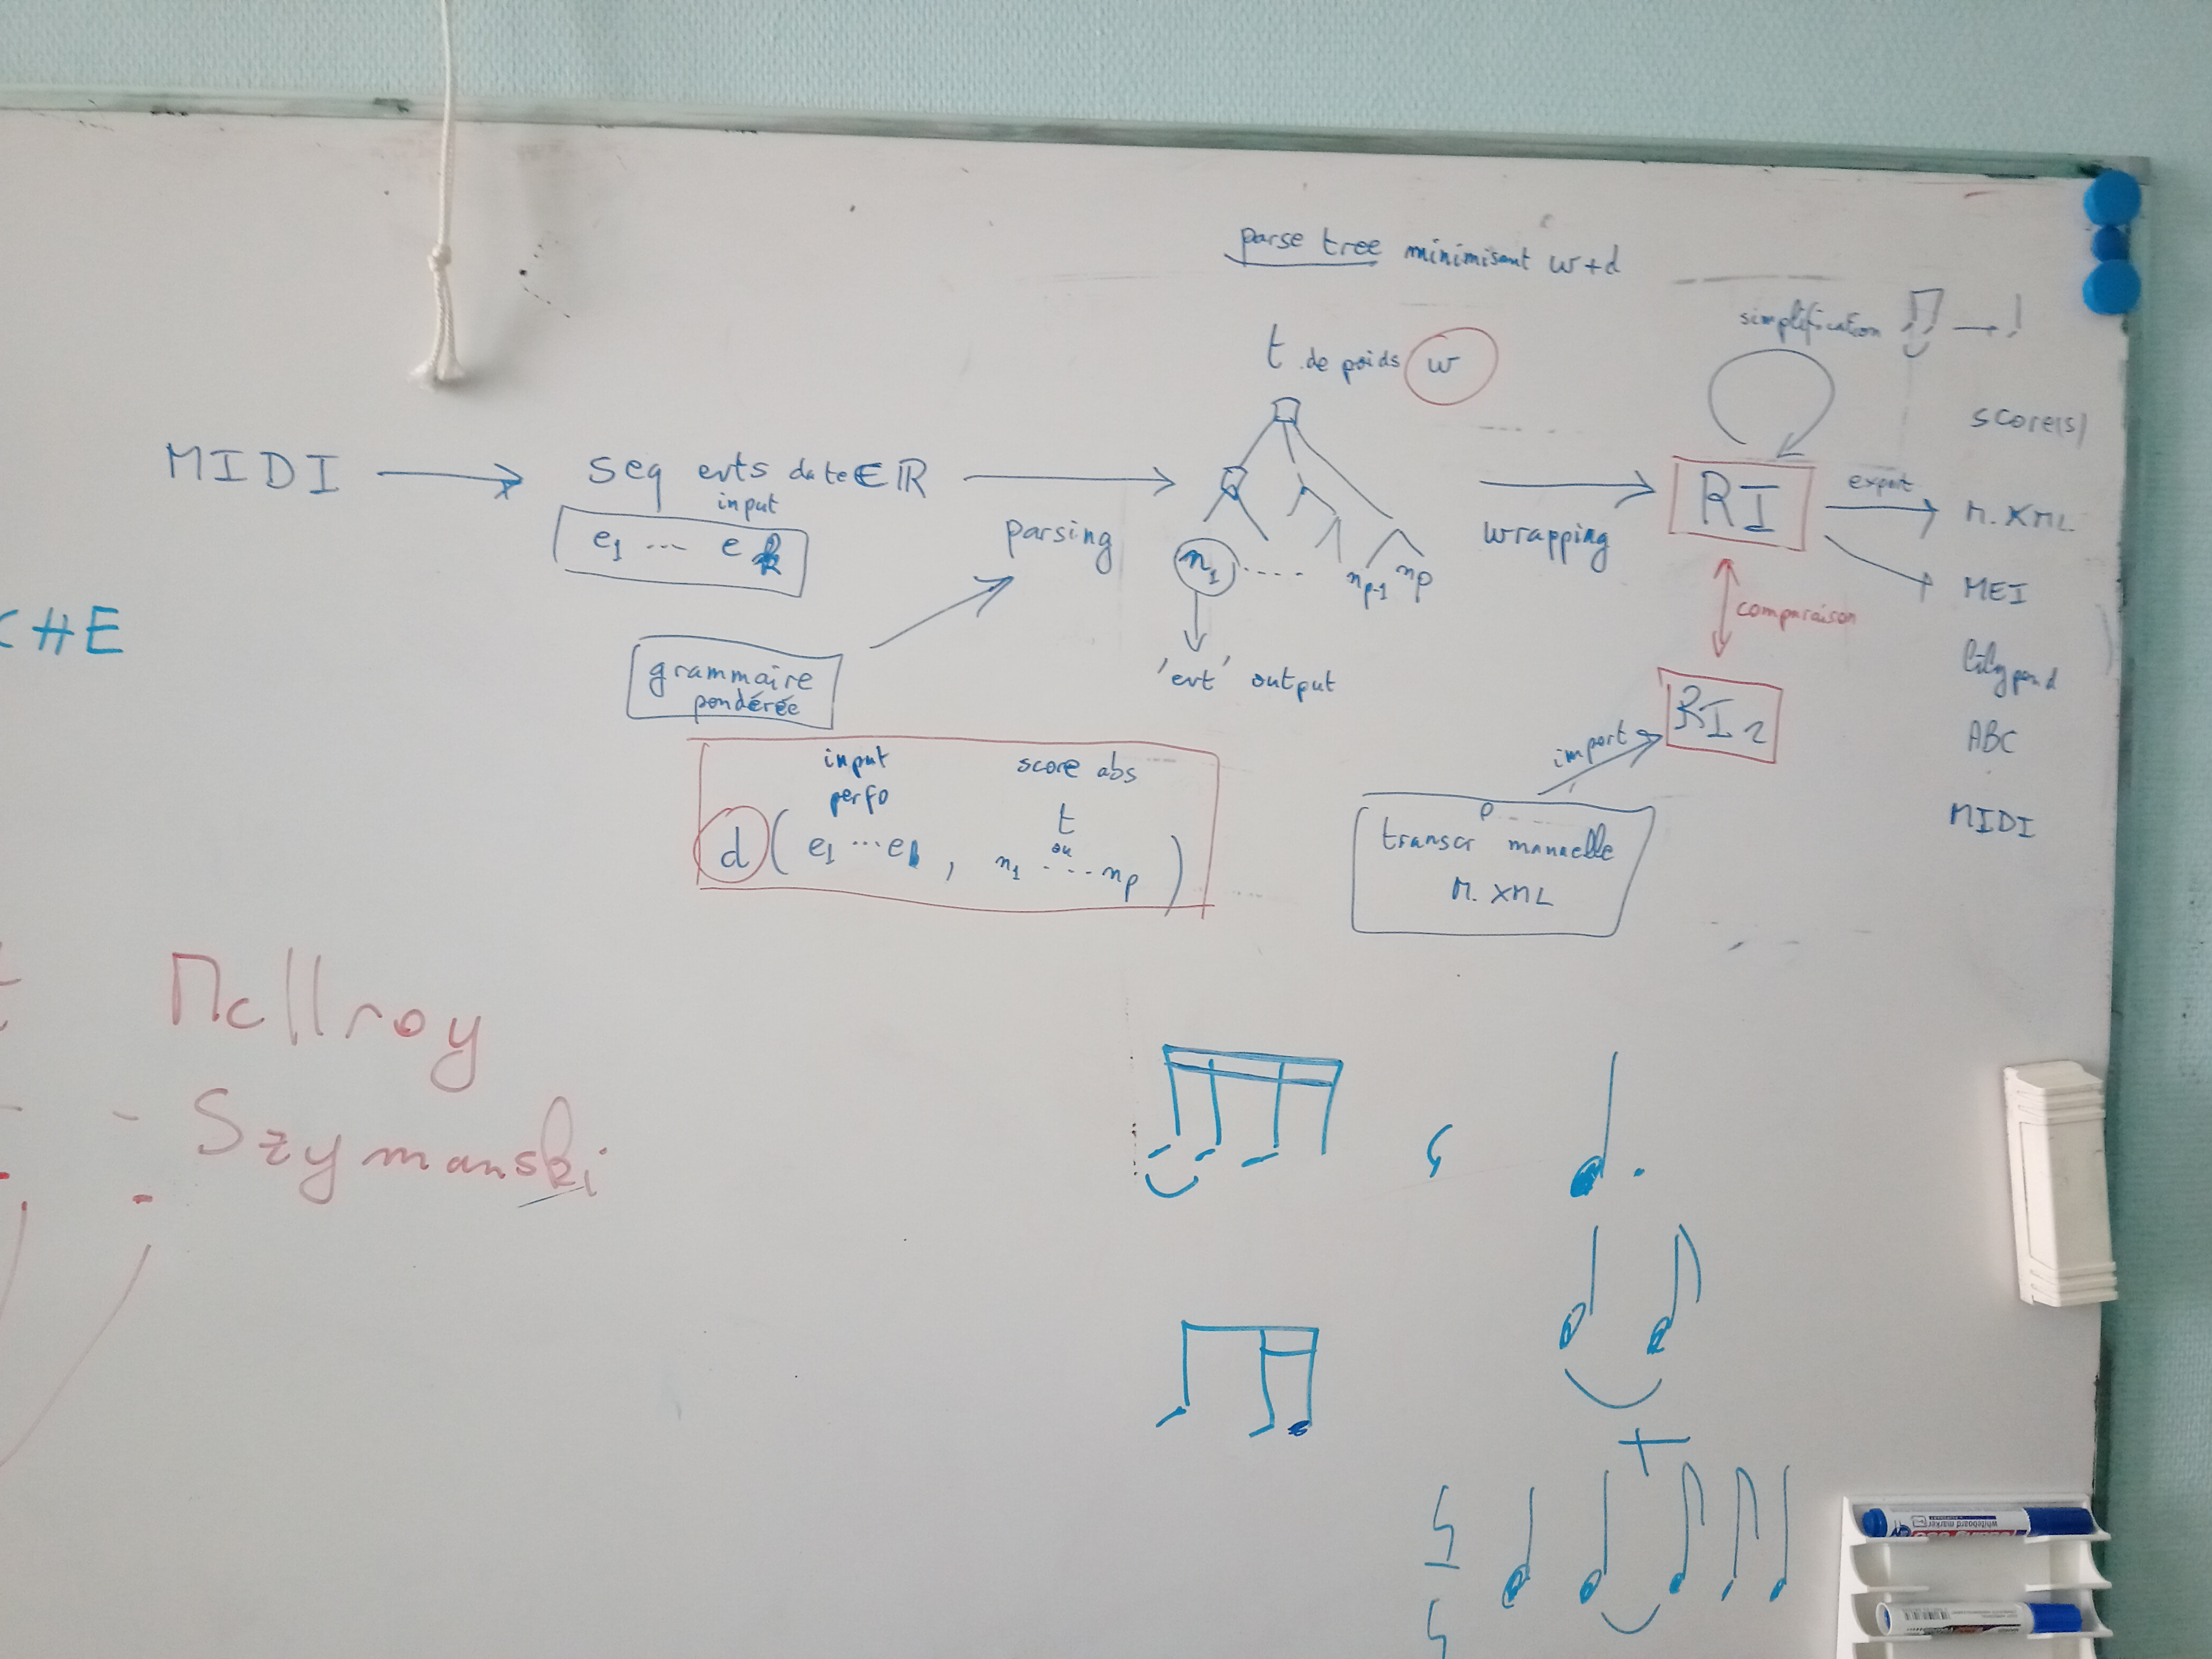
\includegraphics[height=80mm, width=80mm]{images/sujet_stage.jpg} \\\\
	En entrée : midi (séquence d’événements datés (piano roll) accompagné d’une grammaire pondérée)\\
	$\Rightarrow$ parsing\\
	$\Rightarrow$ global parsing tree\\
	$\Rightarrow$ RI (Représentation Intermédiaire) arbres locaux par intruments\\
	$\Rightarrow$ Sortie (xml, mei, lilypond,… )\\
	Minimiser la distance entre le midi et la représentation en arbre.\\\\
	Le but du stage est d’améliorer qparse, un outil de transcription et d’écriture automatique de la batterie (entre autre)\\\\
	\textbf{Le sujet de ce mémoire est de proposer une tâche de reconnaissance du regroupement des notes par les ligatures dans l’écriture de la batterie.}\\\\
	Pour cela, nous utiliserons la logique des systèmes (selon la définition agostinienne).\\$\Rightarrow$ Motif répétitif de plusieurs instruments coordonnées accompagnés d’un texte varié joué par un autre instrument de la batterie.\\\\Nous partirons de propositions génériques de systèmes (environs trois systèmes dans différents style de batterie) que nous tenterons de détecter dans le jeu de données groove.\\\\
	Nous travaillerons aussi sur la détection de répétitions sur plusieurs mesures afin de pouvoir corriger des erreurs sur une des mesures qui aurait dû être identique au autres mais qui présente des différences.
	
	
	

\newpage
\textit{\\En règle générale, l'introduction et la conclusion sont les deux
sections de contenu à ne pas être numérotées. Idéalement, chaque
chapitre commence par une introduction rapide et se termine par une
conclusion rapide pour aider le lecteur à mémoriser et comprendre ce
qui a été fait.}

%%%%%%%%%%%%%%%%%%%%%%%%%%%%%%%%%%%%%%%%%%%%%%%%%%%%%%
%% INTRODUCTION
%%%%%%%%%%%%%%%%%%%%%%%%%%%%%%%%%%%%%%%%%%%%%%%%%%%%%%


\chapter*{Introduction}
\adjustmtc
\addstarredchapter{Introduction} 

\textit{Introduction : présentation générale du contexte et de la
problématique traitée, plan suivi dans le mémoire.}
%% TODO: remplacer ce contenu par le vôtre...
\section*{Présentation générale}

\subsection*{Le contexte}
Ce mémoire de recherche, effectué en parallèle d’un stage à l’Inria dans le cadre du master de traitement automatique des langues de l’Inalco, contient une proposition d’amélioration d’une chaîne de traitement d’ADT de bout en bout.\\
Même si ce sujet ne traite pas directement de langues naturelles, son objet est l’écriture automatique de partitions de musique à partir de données audios. Il nécessite donc la manipulation d’un langage musical codifié avec une grammaire (solfège, durées, nuances, volumes) et soulève de nombreuses problématiques proches de la reconnaissance de la parole.\\\\
\textit{Notes discussion Damien} :\\
\textit{\textbf{Musique} $\Rightarrow$ langue ou langage ? ;\\
\textbf{Partition musicale} $\Rightarrow$ Manière d’écrire la musique…}\\\\
La chaîne de traitement peut-être séparée en deux grandes parties :
\begin{itemize}
	\item Le traitement du signal à partir d’enregistrements audios de performances de batteurs et l’écriture des données sur des fichiers MIDI.
	\item La transformation des fichiers MIDI en partition de batterie (chaque fichier MIDI étant une partition)\\
\end{itemize}

Le sujet du stage se concentre sur la deuxième partie de cette chaîne et le sujet du mémoire est une proposition d’amélioration sur cette partie de la chaîne.

\subsection*{Sujet du stage}
Le but du stage est d’améliorer qparse, un outil de transcription et d’écriture automatique de la batterie (entre autre).\\
L'étude de modèles de langage (LM) incorporant certaines informations musicales de haut niveau nécessaires à la génération de partitions de qualité. On devrait en particulier considérer des hiérarchies d'événements de batterie induisant des placements temporels cohérents et se prêtant à des notations rythmiques faciles à lire pour un batteur entraîné ; voir \cite{foscarin:hal-01988990} pour des modèles structurés en arbre basés sur la théorie formelle du langage, que nous développons dans le contexte d'outils AMT plus généraux.
\subsection*{Ce mémoire}
Le mémoire propose de rechercher de rythmes génériques (\textit{motifs}) en amont dans la chaîne de traitement. Les \textit{motifs} sont prédéfinis avec des combinaisons possibles (\textit{gammes}) qui leur sont associées. Ces \textit{motifs} et leur \textit{gammes} respectives sont appelés \textit{systèmes}.\\L’usage des \textit{systèmes} a pour objectif de fixer des choix le plus tôt possible dans la chaîne de traitement afin de simplifier le reste des calculs en éliminant une partie d’entre eux. Ces choix concernent notamment la métrique, la séparation des voix ainsi que les règles de réécriture.
\subsection*{Problématique traitée}	
	L’écriture musicale offre de nombreuse possibilités d’écriture pour un rythme donné, certains de ces choix sont plus pertinents que d’autres en fonction du contexte.\\
	Reconnaître la métrique d’une partition, la façon de regrouper les notes par les ligatures (séparation des voix), ou simplement le choix pour les différentes continuations possibles (notes pointées, liaisons, silences, etc.) représentent autant de possibilités que de difficultés.
\subsection*{Plan du mémoire}


Introduction générale\\\\
Partie I : Contexte général
\begin{itemize}
	\item État de l’art
	\item La transcription automatique
	\item Les méthodes\\
\end{itemize}
Partie II : Expérimentations
\begin{itemize}
	\item Corpus
	\item Résultats
	\item Discussion\\
\end{itemize}
Conclusion générale\\







%%%%%%%%%%%%%%%%%%%%%%%%%%%%%%%%%%%%%%%%%%%%%%%%%%%%%%%%%%%%%%%%
%% Première partie

\part{Contexte général}



%%%%%%%%%%%%%%%%%%%%%%%%%%%%%%%%%%%%%%%%%%%%%%%%%%%%%%
%% ÉTAT DE L'ART
%%%%%%%%%%%%%%%%%%%%%%%%%%%%%%%%%%%%%%%%%%%%%%%%%%%%%%

%% Nota Bene : il est possible de stocker chaque chapitre dans un
%% fichier *.tex distinct (par exemple pour ce chapitre, de la
%% commande \chapter{} jusqu'à la conclusion de ce chapitre) nommé,
%% par exemple "chapitre-etat-art.tex" qui sera appelé au moyen de la
%% commande suivante (la compilation du fichier *.tex principal
%% compile automatiquement les fichiers inclus) :
%%
%% \include{chapitre-etat-art}

\chapter{\'Etat de l'art}
\label{chap:articles}

%% Ajustement de la mini table des matières du fait de l'introduction
%% non numérotées qui introduit un décalage
\adjustmtc
\minitoc

\textit{\\L’état de l'art (chapitre~\ref{chap:articles})~: les articles
qui traitent du même sujet que vous, présentés en un tout cohérent
\emph{(extraire de chaque article lu les points essentiels et
	présenter dans ce chapitre le résultat de ces lectures en
	regroupant les articles par point essentiel)}}
\section{La musique et le TAL}
Aborder la musique à travers le TAL nécessite une réflexion autour de la musique en tant que langage ainsi que la possibilité de comparer ce même langage avec les langues naturelles. Quelques travaux en neuroscience ont abordé la question, notamment par observation des processus cognitifs et neuronaux que les systèmes de traitement de ces deux langages avaient en communs. Dans le travail de Poulin-Charronnat et al. \cite{poulincharronnat:hal-01985213}, la musique est reconnue comme étant un système complexe spécifique à l’être humain dont une des similitudes avec les langues naturelles est l’émergence de régularités reconnues implicitement par le système cognitif. La question de la pertinence de l’analogie entre langues naturelles et langage musical a également été soulevée à l’occasion de projets de recherche en TAL. Keller et al. \cite{keller:hal-03279850} ont exploré le potentiel de ces techniques à travers les plongements de mots et le mécanisme d’attention pour la modélisation de données musicales. La question du sens d’une phrase musicale apparaît, selon eux, à la fois comme une limite et un défi majeur pour l’étude de cette analogie.\\
D’autre travaux très récents, ont aussi été révélé lors de la \textit{première conférence sur le NLP pour la musique et l'audio (NLP4MusA 2020)}. Lors de cette conférence, Jiang et al. \cite{Jiang2020DiscoveringMR} ont présenté leur implémentation d’un modèle de langage musical auto-attentif visant à améliorer le mécanisme d'attention par élément, déjà très largement utilisé dans les modèles de séquence modernes pour le texte et la musique.
\section{La transcription automatique de la musique}
L'objectif de la transcription automatique de la musique (AMT) \cite{article1} est de convertir la performance d'un musicien en notation musicale - un peu comme la conversion de la parole en texte dans le traitement du langage naturel. Bien que l’AMT soit un domaine de recherche en plein essor dans lequel plusieurs approches différentes sont encore activement étudiées, les performances des systèmes actuels ne sont pas encore suffisantes pour certaines applications qui exigent un haut degré de précision \cite{article1}. Même si les applications typiques de l'AMT comprennent l'estimation de la multi-tonalité, la classification des genres musicaux, la détection du début et de la fin des notes de musique, l'estimation du tempo, le suivi du rythme et la transcription de la musique. La plupart des travaux se sont concentrés sur le traitement du signal vers la génération du midi \cite{article2}. Seuls quelques travaux récents \cite{foscarin:hal-01988990} s’intéressent de près à la création d’outils permettant la génération de partition. Les applications de l’AMT ont aussi de la valeur dans les domaines oraux ou d’improvisation qui manquent de partition (jazz, pop) \cite{article1}. Les applications de l’ADT serait utile pour ces styles de musiques puisque la batterie y est amplement représentée.
\section{La transcription automatique de la batterie} 
Un grand nombre travaux ont déjà été menés dans le domaine de l’ADT. La plupart ont été énumérés par Wu et al. \cite{8350302} qui, pour mieux comprendre la pratique des systèmes d’ADT, se concentrent sur les méthodes basées sur la factorisation matricielle non négative et celles utilisant des réseaux neuronaux récurrents.\\
La batterie a un statuts à part dans l’univers de l’AMT puisqu'il s'agit d'instruments sans hauteur, d'événements auxquels une durée est rarement attribuée et de notations spécifiques (par exemple sur les têtes de notes). Si les ordinateurs étaient capables d'analyser la partie de la batterie dans la musique enregistrée, cela permettrait une variété de tâches de traitement de la musique liées au rythme. En particulier, la détection et la classification des événements sonores de la batterie par des méthodes informatiques est considérée comme un problème de recherche important et stimulant dans le domaine plus large de la recherche d'informations musicales \cite{8350302}. Cependant, la plupart des travaux déjà entrepris se concentrent sur des méthodes de calcul pour la détection d'événements sonores de batterie à partir de signaux acoustiques ou sur la séparation entre les évènement sonore de batterie avec ceux des autres instruments dans un orchestre ou un groupe de musique \cite{2802}, ainsi que sur l'extraction de caractéristiques de bas niveau telles que la classe d'instrument et le moment de l'apparition du son. Très peu d'entre eux ont abordé la tâche de générer des partitions de batterie.
%\section{Introduction}
%Dans ce chapitre, nous présentons...
%
%\section{Contenu}
%Une section dans ce chapitre avec un appel cliquable de référence
%%bibliographique~\cite{grouin-2014jbi}.
%
%\section{Conclusion}
%Conclusion de ce chapitre.


%%%%%%%%%%%%%%%%%%%%%%%%%%%%%%%%%%%%%%%%%%%%%%%%%%%%%%
%% MÉTHODES
%%%%%%%%%%%%%%%%%%%%%%%%%%%%%%%%%%%%%%%%%%%%%%%%%%%%%%


\chapter{Méthodes}
\label{chap:methodes}
\minitoc

\textit{\\Méthodes (chapitre~\ref{chap:methodes})~: les méthodes
appliquées, avec le détail des expériences réalisées (différentes
configurations)~;}

\textit{\\Corpus (chapitre~\ref{chap:corpus})~: le corpus utilisé
	\emph{(caractéristiques, pré-traitements appliqués)}}

\section{Introduction}
Dans ce chapitre...
\subsection{Chaîne de traitement}
\begin{itemize}
	\item Reconnaître un motif (système) dans une partition (un fichier midi)\\
	Sur une mesure de l’input $\Rightarrow$ Motif (système) reconnu : true ou false
	\item Si true : 
	\begin{itemize}
		\item Séparer les voix
		\item Simplifier l’écriture de chaque voix\\\\
	\end{itemize}
\end{itemize}
Chaîne de traitement :\\
if match(system\_parse\_tree(system + pitch), input\_midi\_parse\_tree)\\
\tab then voice\_split ;\\
\tab for voice in voice\_split:\\
\tab \tab simplication voice

\subsection*{Les sytèmes en batterie}
SYSTÈME ==> MOTIF (2-3 instruments sur 1-2 voix, joué en boucle) + TEXTE (1 instrument sur 1 voix, irrégulier)\\
ex : système afro-cubain, trois voix.
Proposition pour la détection de la direction des hampes et pour les ligatures (regroupement des notes et séparation des voix.)
\begin{itemize}
	\item \textbf{\textit{Les systèmes :}}\\
	$\Rightarrow$ Un système est la combinaison d’un ou plusieurs éléments qui jouent un rythme en boucle (système) et d’un autre élément qui joue un \textit{texte} rythmique variable mais respectant les règles propre au système (texte).\\
	Définition d’un système :\\
	
	En cas de système, les ligatures forment deux voies :
	\begin{itemize}
		\item Le texte ;
		\item Le système.
	\end{itemize}
	\textit{Mettre des exemples de différents systèmes.}
	\item \textbf{\textit{Les moulins :}}\\
	Lorsqu’il y a plus d’une voie, ils sont prioritaires pour les ligatures.\\
	\textit{Mettre des exemples.}\\
\end{itemize}
\subsection*{Gestion des silences et des têtes de notes}
Rythme tree (RT)\\
- Le symbole "-" est une continuation (liaison) mais pour une partition de
batterie, ça serait un silence par défaut sauf peut-être pour les ouvertures
de charley et éventuellement les cymbales ou un tom basse qui résonne.\\
$\Rightarrow$ Question de la (notation noir + silence) vs blanche.\\
$\Rightarrow$ On privilégierait (noir + silence) puisque les symboles « x » des cymbales ne
peuvent pas porter d’indication de durée dans la tête de notes.\\
Les 3 parties d’une note :
\begin{itemize}
	\item durée
	\item hampe
	\item tête de note (peut aussi indiquer la durée mais en batterie on évitera les blanches, etc.)
\end{itemize}
source : \url{https://fr.wikipedia.org/wiki/Note_de_musique}\\\\
\subsection*{Définition des têtes de notes et des hauteurs}
\subsubsection*{Proposition de définition d’un standard de départ}
Pour la transcriptions, nous proposons de choisir la base Agostini. La caisse claire centrale sur la portée est aussi centrale sur la batterie est elle est un élément qui conditionne la position des jambes (écart entre les pédales, etc.) ainsi que l’organisation des éléments en hauteur (toms, cymbales, etc.).
On pensera en terme de symétrie la répartition des éléments par rapport au point central que constitue la caisse claire.\\
Cette symétrie s’opère en trois dimensions :
\begin{itemize}
	\item Les hauteurs en terme de fréquences ;
	\item La hauteur physique des éléments :\\
	Du bas vers le haut : pédales, toms et caisse, cymbales
	\item L’ergonomie, qui hiérarchise l’importance des éléments sur la portée (caisse claire au centre, hh-pied et ride sont aux deux extrémités).
\end{itemize}

%\section*{Installation de cmake-3.20.4}
Installation de CMake et d’un environnement C++ pour Vim.\\\\
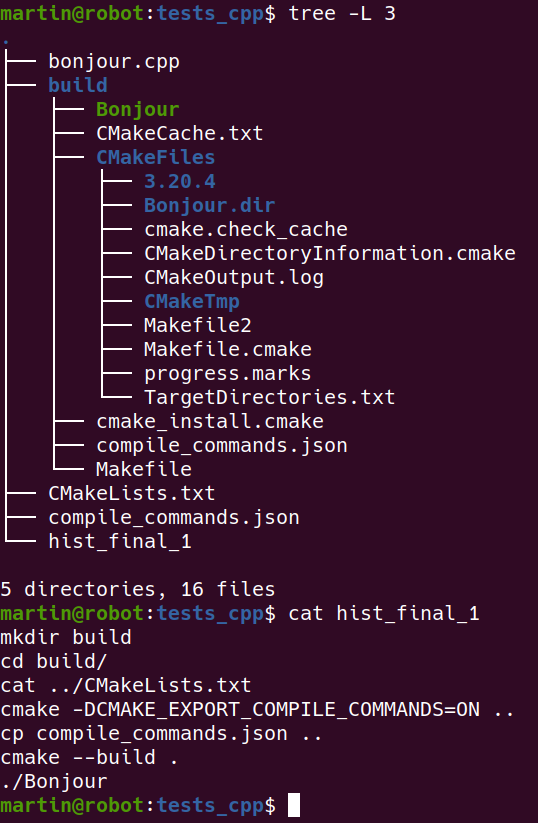
\includegraphics[height=70mm, width=50mm]{images/cpp_env_0.png}\\\\
- Lire sur la réécriture : 1\_articles/1\_rt\_representation\\
- Lire Qparse : \url{https://qparse.gitlabpages.inria.fr/}\\\\
qparse (version beta) entrée MIDI (groove), sortie MIDI (modifiée) ou
partition MEI.
\newpage

\section{Représentations, systèmes et réécriture}
\subsection{La notation de la batterie}
\subsubsection{La hauteur des notes et les têtes de notes}
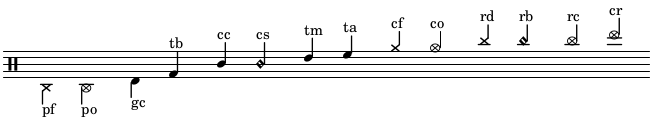
\includegraphics[height=30mm, width=155mm]{z_images/1_description_notation/notes.png}
partition 1
\subsubsection{Les nuances}
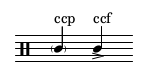
\includegraphics[height=20mm, width=35mm]{z_images/1_description_notation/nuances.png}\\
partition 2\\\\
Bien expliquer les accents, remplacer p et f par g et a\\
$\Rightarrow$ nuance VS articulation\\
\subsubsection{La séparation des voix}
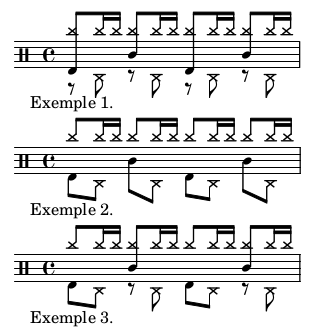
\includegraphics[height=65mm, width=60mm]{z_images/1_description_notation/separation/0_exemples_separation.png}\\
partition 3
\subsection{La notation midi de la batterie}
\subsubsection{Représentation symbolique (MIDI)}
………\\
\subsubsection{Les pitchs et la vélocité}
\begin{table}[h]
	\centering
	\begin{tabular}{|c|c|c|} \hline
		Codes & Instruments & Pitchs \\ \hline
		cf & charley-main-fermé & 22, 42 \\
		co & charley-main-ouvert & 26 \\
		pf & charley-pied-fermé & 44 \\
		rd & ride & 51 \\
		rb & ride-cloche (bell) & 53 \\
		rc & ride-crash & 59 \\
		cr & crash & 55 \\
		cc & caisse-claire & 38, 40 \\
		cs & cross-stick & 37 \\
		ta & tom-alto & 48, 50 \\
		tm & tom-medium & 45, 47 \\
		tb & tom-basse & 43, 58 \\
		gc & grosse-caisse & 36 \\ \hline
	\end{tabular}
	\caption{Pitchs et instruments}
	%	\label{tab:exemple}
\end{table}
\begin{table}[h]
	\centering
	\begin{tabular}{|c|c|c|c|} \hline
		Codes & Instruments & Pitchs & Vélocité \\ \hline
		cop & charley-main-ouvert & 46 & ? \\ \hline
	\end{tabular}
	\caption{Vélocité et nuances}
\end{table}
Pas de charley pied ouvert…
Nous ne prendrons en compte la vélocité que pour la cc, les toms et les cymbales jouées aux mains. Les nuances de grosse caisse et charley aux pieds sont le plus souvent insignifiantes, elles ne sont marquées sur le figure qu’à titre indicatif.\\\\
Si la vélocité est en dessous de 40, il s’agit de ghost-notes : la tête de note devra être entouré de parenthèses et le suffixe \textit{p (piano)} devra être ajouté au codes de l’instrument. (Voir ccp ci-dessus.)\\\\
Si la vélocité est au dessus de 90, il s’agit de notes accentuées : le symbole « > » et le suffixe \textit{f (forte)} devra être ajouté au codes de l’instrument. (Voir ccf ci-dessus.)\\\\
Lorsque la vélocité va de 40 à 89, on considèrera le volume comme normal et aucun symbole supplémentaire ne sera ajouté à la note.\\\\
L’instrument qui sera difficile à placer sera la caisse claire car elle ne sera pas toujours affiliée aux mêmes instruments.
\subsubsection{Les dilemmes}
Le charley de pitch 46 est considéré comme le charley ouvert joué à la main sur le haut de la cymbale mais souvent, ça correspond au geste « tranche-olive » de la baguette lorsque le batteur accentue avec la tranche et joue moins fort avec l’olive sur le plat de la cymbale. Je vais dans un premier temps considérer le pitch comme \textbf{charley-main-ouvert-piano} (ghost-note)
\newpage
\subsubsection{Représentations en arbres}
Voici une représentation de la \textit{partition 3} en arbre de rythme avec les codes de chaque instrument :\\\\
\Tree[ [ [rd\\gc ][ [rd\\pf ][rd ]]]
[ [rd\\cc ][ [rd\\pf ][rd ]]]
[ [rd\\gc ][ [rd\\pf ][rd ]]]
[ [rd\\cc ][ [rd\\pf ][rd ]]] ]\\\\\\
Ci-dessous, le même arbre dont les codes des instruments sont remplacés par leurs données midi respectives :\\\\
\Tree[ [ [51\\36 ][ [51\\44 ][51 ]]]
[ [51\\38 ][ [51\\44 ][51 ]]]
[ [51\\36 ][ [51\\44 ][51 ]]]
[ [51\\38 ][ [51\\44 ][51 ]]] ]\\\\\\
Cet arbre représente un rythme unique dont les possiblités de notation sur une partition sont théoriquement multiples.(Voir \textit{partition 3}).\newpage
\subsection{Les systèmes}
\subsubsection{Définition}

Système = motif + texte
motif = rythmes coordonné joués en boucle
texte = rythme irrégulier joué avec un seul membre.\\

trois système standard :
\begin{itemize}
	\item binaire
	\item ternaire (shuffle, afro, rock)
	\item jazz
	\item afro-cubain
\end{itemize}

\subsubsection{Utilité}
\begin{itemize}
	\item Séparation des voix
	\item Définir une métrique
	\item Conditionner des règles spécifiques de réécriture
\end{itemize}
\ \\
Créer un ensemble de systèmes :
\begin{itemize}
	\item 4/4 binaire FAIT
	\item jazz vs ternaire(12/8)
	\item afro-cubain (trois voix ??)
	\item Tout transcrire avec lilypond et en arbres d’analyse syntaxique.
	\item Créer les arbres de voix séparées.
	\item Créer les arbres de voix séparées simplifiés (rewriting).\\	
\end{itemize}

Pour la \textbf{séparation des voix} et la \textbf{définition des métriques}, nous nous intéresserons principalement à la partie \textit{motif} des systèmes qui seront présentés. La partie \textit{texte} nous intéressera plus pour les \textbf{combinaisons de réécritures}.
\newpage
\subsubsection{Pour la séparation des voix}
\textbf{Motif 4-4 binaire}\\\\
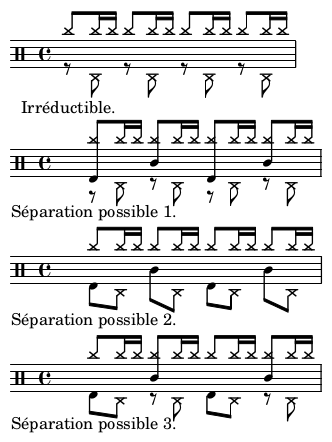
\includegraphics[height=100mm, width=70mm]{z_images/1_description_notation/separation/separation_0.png}\\\\
Ici, le système est construit sur un modèle rock en 4/4 : after-beat sur les 2 et 4 avec un choix de répartition des cymbales type fast-jazz. Le système est constitué par défaut du motif ride/ch-pf/cc et d’un texte joué à la grosse-caisse. La troisième séparation proposée est privilégiée car elle répartit selon 2 voix, une voix pour les mains (ride + cc) et une voix pour les pieds (ch-pf + gc). Ce choix paraît plus équilibré car deux instruments sont utilisés par voix et plus logique pour le lecteur puisque les mains sont en haut et les pieds en bas.\\
D’autres choix d’écriture auraient été possibles :
\begin{itemize}
	\item Toutes les hampes en haut ;
	\item Combinaison motif 1 et 2 en donnant 2 directions aux hampes de la cc).\\
\end{itemize}
\newpage
\textbf{Motif 4-4 jazz}\\\\
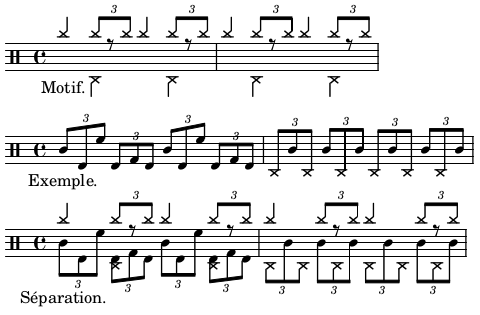
\includegraphics[height=65mm, width=100mm]{z_images/1_description_notation/separation/separation_1.png}\\\\
Dans la plupart des méthodes, le charley n’est pas écrit car considéré comme évident en jazz traditionnel. Ce qui facilite grandement l’écriture : la ride et les crash sur la voix du haut et le reste sur la voix du bas. Ici, le partie prit et de tout écrire. Dans l’exemple ci-dessus, les mesures 1 et 2 combinées avec le \textit{motif} de la première ligne, sont des cas typiques de la batterie jazz. Tout mettre sur la voix haute serait surchargé. De plus, la grosse caisse entre très souvent dans le flot des combinaisons de toms et de caisse claire et son écriture séparée serait inutilement compliquée et peu intuitive pour le lecteur. Le choix de séparation sera donc de laisser les cymbales en haut et toms, caisse-claire, grosse-caisse et pédale de charley en bas.\\\\

\textbf{Système 4-4 afro-cubain}\\\\
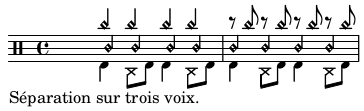
\includegraphics[height=25mm, width=80mm]{z_images/1_description_notation/separation/separation_2.png}\\\\

\subsubsection{Pour la reconnaissance de la métrique}

\textit{\textbf{12/8 vs 4/4 ternaire}}\\\\
\textbf{Motif 12/8}\\\\
%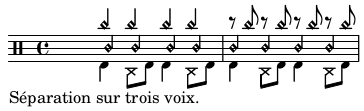
\includegraphics[height=30mm, width=100mm]{z_images/1_description_notation/separation/separation_2.png}\\\\
\newpage

\subsubsection{Construction des systèmes pour les expérimentations}
\textbf{Textes pour les systèmes en 4/4 binaire}\\\\
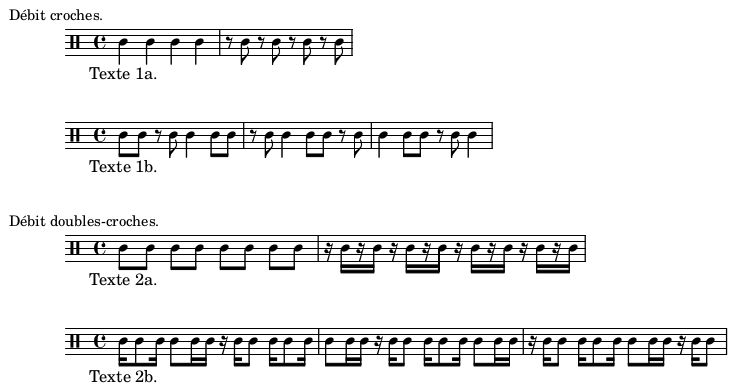
\includegraphics[height=65mm, width=100mm]{z_images/1_description_notation/systemes/textes_4-4_binaires.png}\\\\
\textbf{Motifs pour les systèmes en 4/4 binaire}\\\\
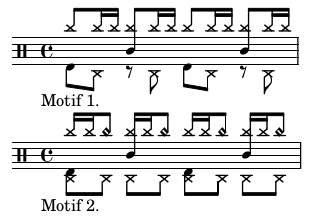
\includegraphics[height=30mm, width=50mm]{z_images/1_description_notation/systemes/motifs_4-4_binaires.png}\newpage
\textbf{Systèmes résultants}\\\\
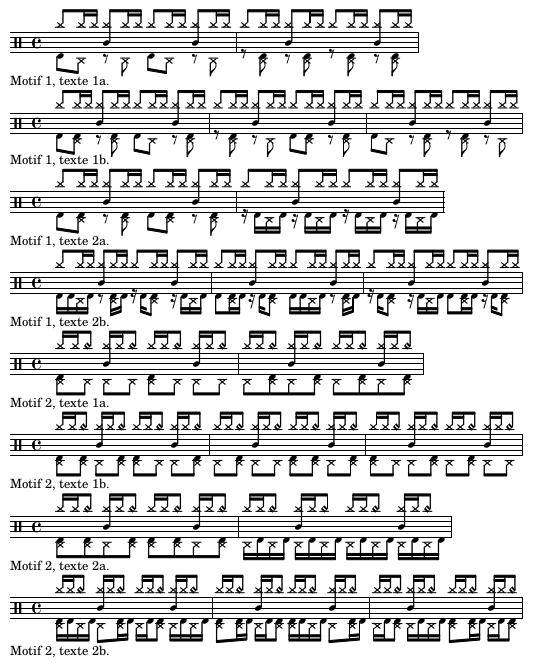
\includegraphics[height=120mm, width=100mm]{z_images/3_experimentations/experience_1/systemes_recherches.png}
%% stock

\newpage
À partir de ce choix d’écriture, le système suivant est défini :\\\\
%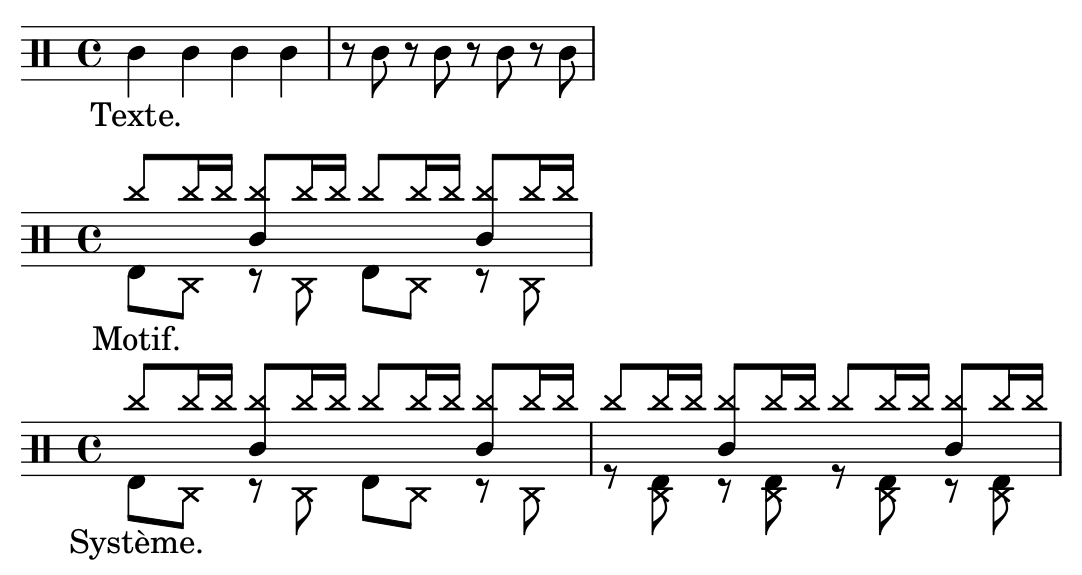
\includegraphics[height=65mm, width=115mm]{z_images/3_experimentations/system_drummer_01_session1_004.png}\\
%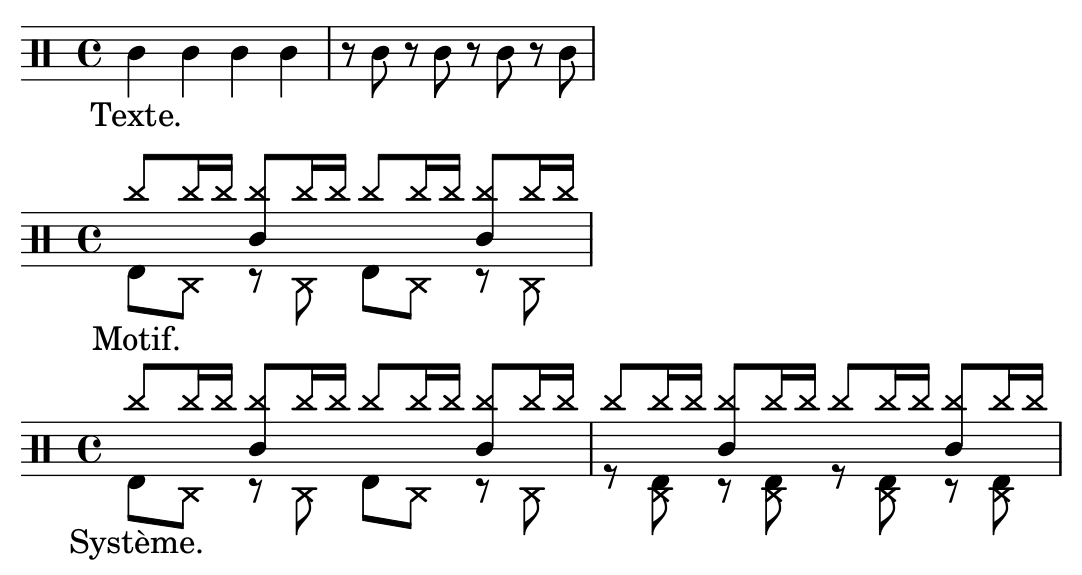
\includegraphics[height=65mm, width=115mm]{z_images/3_experimentations/system_drummer_01_session1_004.png}\\
Dans le motif, la grosse caisse est notée car elle fait partie de l’équilibre musical de ce rythme mais rigousement, elle ne devrait pas y apparaître puisque qu’elle sera indiquée par le texte.\\
Dans ce système, les noires ne doivent jamais tomber en même temps que les caisse-claires, donc, quand le texte donnera des noires sur les deuxièmes et quatrièmes temps, elles ne seront jamais jouées par le batteur (exemple sur la première mesure du système).\\


Voici la représentation de ce système en arbre de rythme :\\

\resizebox{420pt}{!}{\Tree[.Système [.Mesure\ 1  [.Temps\ 1 [51\\36 ][ [51\\44 ][51 ]]]
	[.Temps\ 2 [51\\38 ][ [51\\44 ][51 ]]]
	[.Temps\ 3 [51\\36 ][ [51\\44 ][51 ]]]
	[.Temps\ 4 [51\\38 ][ [51\\44 ][51 ]]] ]
	[.Mesure\ 2 [.Temps\ 1 [51 ][ [51\\44\\36 ][51 ]]]
	[.Temps\ 2 [51\\38 ][ [51\\44\\36 ][51 ]]]
	[.Temps\ 3 [51 ][ [51\\44\\36 ][51 ]]]
	[.Temps\ 4 [51\\38 ][ [51\\44\\36 ][51 ]]] ]]}\\

\subsubsection{Séparation des voix}
\resizebox{430pt}{!}{\Tree[.Voix\ haute 
	[.Mesure\ 1 
	[. [rd ][. [rd ][rd ]]]
	[. [rd\\cc ][. [rd ][rd ]]]
	[. [rd ][. [rd ][rd ]]]
	[. [rd\\cc ][. [rd ][rd ]]] ]
	[.Mesure\ 2 
	[. [rd ][. [rd ][rd ]]]
	[. [rd\\cc ][. [rd ][rd ]]]
	[. [rd ][. [rd ][rd ]]]
	[. [rd\\cc ][. [rd ][rd ]]] ]]}\\\\\\
\resizebox{400pt}{!}{\Tree[.Voix\ basse 
	[.Mesure\ 1 
	[. [gc ][. [pf ][tie ]]]
	[. [tie ][. [pf ][tie ]]]
	[. [gc ][. [pf ][tie ]]]
	[. [tie ][. [pf ][tie ]]] ]
	[.Mesure\ 2 
	[. [tie ][. [pf\\gc ][tie ]]]
	[. [tie ][. [pf\\gc ][tie ]]]
	[. [tie ][. [pf\\gc ][tie ]]]
	[. [tie ][. [pf\\gc ][tie ]]] ]]}

\subsubsection{Réécriture (Simplification)}
\resizebox{400pt}{!}{\Tree[.Voix\ basse 
	[.Mesure\ 1 
	[. [gc ][pf ]]
	[. [tie ][pf ]]
	[. [gc ][pf ]]
	[. [tie ][pf ]] ]
	[.Mesure\ 2 
	[. [tie ][pf\\gc ]]
	[. [tie ][pf\\gc ]]
	[. [tie ][pf\\gc ]]
	[. [tie ][pf\\gc ]] ]]}\\\\
La voix haute reste inchangée.
%preamble:
%
%
%%\usetikzlibrary{backgrounds}
%%\usetikzlibrary{trees}
%
%
%Figure 1:
%
%\begin{figure}
%\centering
%\begin{subfigure}
%[$\frac{1}{2} \frac{1}{4} \frac{1}{4}$]
%{
%\begin{tabular}{c}
%%\includegraphics[scale=\scorescale]{images/1a.png}\\
%\begin{tikzpicture} [-,thick]
%\tikzstyle{level 1}=[level distance=7mm,sibling distance=6mm]
%\tikzstyle{level 2}=[level distance=7mm,sibling distance=5mm]
%\node {$\deux$}
%  child { node {$\note$} }
%  child { node {$\deux$}
%    child { node {$\note$} }
%    child { node {$\note$} } };
%\end{tikzpicture}
%\end{tabular}
%%\label{fig:subfig1a}}
%%
%\hspace{0.6cm}
%\begin{subfigure}
%[$\lbrack \frac{1}{6} \rbrack\, \frac{1}{6}\,
%  \lbrack \frac{1}{6} \rbrack\, \frac{1}{6}\,
%  \lbrack \frac{1}{6} \rbrack\, \frac{1}{6}$]
%{
%\begin{tabular}{c}
%%\includegraphics[scale=\scorescale]{images/1b.png}\\
%\begin{tikzpicture} [-,thick]
%\tikzstyle{level 1}=[level distance=7mm,sibling distance=9mm]
%\tikzstyle{level 2}=[level distance=7mm,sibling distance=5mm]
%\node {$\trois$}
%  child { node {$\deux$}
%    child { node {$\rest$} }
%    child { node {$\note$} } }
%  child { node {$\deux$}
%    child { node {$\rest$} }
%    child { node {$\note$} } }
%  child { node {$\deux$}
%    child { node {$\rest$} }
%    child { node {$\note$} } };
%\end{tikzpicture}
%\end{tabular}
%%\label{fig:subfig1b}}
%%
%\hspace{0.6cm}
%\subfig
%[$\frac{1}{5} \frac{1}{5}
%  \frac{1}{15}\frac{1}{15}\frac{1}{15}
%  \frac{1}{5} \frac{1}{5}$]
%{
%\begin{tabular}{c}
%%\includegraphics[scale=\scorescale]{images/1c.png}\\
%\begin{tikzpicture} [-,thick]
%\tikzstyle{level 1}=[level distance=7mm,sibling distance=5mm]
%\tikzstyle{level 2}=[level distance=7mm,sibling distance=5mm]
%\node {$\cinq$}
%  child { node {$\note$} }
%  child { node {$\note$} }
%  child { node {$\trois$}
%    child { node {$\note$} }
%    child { node {$\note$} }
%    child { node {$\note$} } }
%  child { node {$\note$} }
%  child { node {$\note$} } ;
%\end{tikzpicture}
%\end{tabular}
%\label{fig:subfig1c}}
%%
%\begin{RR}
%\hspace{0.6cm}
%\subfig
%[$\frac{1}{12} \frac{1}{12} \frac{1}{12} \frac{1}{12} \frac{1}{3}
%\frac{1}{12} \frac{1}{12} \frac{1}{12} \frac{1}{12}$]
%{
%\begin{tabular}{c}
%%\includegraphics[scale=0\scorescale]{images/1d.png}\\
%%\hspace{0.3cm}
%\begin{tikzpicture} [-,thick]
%\tikzstyle{level 1}=[level distance=7mm,sibling distance=9mm]
%\tikzstyle{level 2}=[level distance=6mm,sibling distance=8mm]
%\tikzstyle{level 3}=[level distance=6mm,sibling distance=5mm]
%\node {$\trois$}
%  child { node {$\deux$}
%    child { node {$\deux$}
%      child { node {$\note$} }
%  child { node {$\note$} } }
%    child { node {$\deux$}
%      child { node {$\note$} }
%  child { node {$\note$} } } }
%  child { node {$\note$} }
%  child { node {$\deux$}
%    child { node {$\deux$}
%      child { node {$\note$} }
%  child { node {$\note$} } }
%    child { node {$\deux$}
%      child { node {$\note$} }
%  child { node {$\note$} } } };
%\end{tikzpicture}
%\end{tabular}
%\label{fig:subfig1d}}
%\end{RR}
%\caption{Simple trees of $\T(\Sigmar)$ with their corresponding
%rhythmic notations and values.}
%\label{fig:trees0}
%\end{figure}
%\subsection*{Tests avec qtree}
[…]\\

%\Tree[.IP [.NP [.Det \textit{the} ]
%               [.N\1 [.N \textit{package} ]]]
%          [.I\1 [.I \textsc{3sg.Pres} ]
%                [.VP [.V\1 [.V \textit{is} ]
%                           [.AP [.Deg \textit{really} ]
%                                [.A\1 [.A \textit{simple} ]
%                                      \qroof{\textit{to use}}.CP ]]]]]]
%                                      
%\Tree[. [. [.rd\\gc ][. [rd\\chpf ][rd ]]]
%        [. [.rd\\cc ][. [rd\\chpf ][rd ]]]
%        [. [.rd\\gc ][. [rd\\chpf ][rd ]]]
%        [. [.rd\\cc ][. [rd\\chpf ][rd ]]] ]
%Voix haute (Les mesure 1 et 2 sont identiques) :\\\\
%\Tree[. [. [rd ][. [rd ][rd ]]]
%        [. [rd\\cc ][. [rd ][rd ]]]
%        [. [rd ][. [rd ][rd ]]]
%        [. [rd\\cc ][. [rd ][rd ]]] ]\\\\\\
%Voix basse (mesure 1) :
%\Tree[. [. [gc ][. [pf ][$\emptyset$ ]]]
%        [. [$\emptyset$ ][. [pf ][$\emptyset$ ]]]
%        [. [gc ][. [pf ][$\emptyset$ ]]]
%        [. [$\emptyset$ ][. [pf ][$\emptyset$ ]]] ]\\
%Voix basse (mesure 2) :
%\Tree[. [. [$\emptyset$ ][. [pf\\gc ][$\emptyset$ ]]]
%		[. [$\emptyset$ ][. [pf\\gc ][$\emptyset$ ]]]
%		[. [$\emptyset$ ][. [pf\\gc ][$\emptyset$ ]]]
%		[. [$\emptyset$ ][. [pf\\gc ][$\emptyset$ ]]] ]\\\\\\
%\resizebox{420pt}{!}{\Tree[.Voix\ haute 
%	[.Mesure\ 1 
%			[. [rd ][. [rd ][rd ]]]
%			[. [rd\\cc ][. [rd ][rd ]]]
%			[. [rd ][. [rd ][rd ]]]
%			[. [rd\\cc ][. [rd ][rd ]]] ]
%	[.Mesure\ 2 
%			[. [rd ][. [rd ][rd ]]]
%			[. [rd\\cc ][. [rd ][rd ]]]
%			[. [rd ][. [rd ][rd ]]]
%			[. [rd\\cc ][. [rd ][rd ]]] ]]}
%\resizebox{420pt}{!}{\Tree[.Voix\ basse 
%	[.Mesure\ 1 
%	       [. [gc ][. [pf ][$\emptyset$ ]]]
%	       [. [$\emptyset$ ][. [pf ][$\emptyset$ ]]]
%	       [. [gc ][. [pf ][$\emptyset$ ]]]
%	       [. [$\emptyset$ ][. [chpf ][$\emptyset$ ]]] ]
%	[.Mesure\ 2 
%	       [. [$\emptyset$ ][. [pf\\gc ][$\emptyset$ ]]]
%	       [. [$\emptyset$ ][. [pf\\gc ][$\emptyset$ ]]]
%	       [. [$\emptyset$ ][. [pf\\gc ][$\emptyset$ ]]]
%	       [. [$\emptyset$ ][. [pf\\gc ][$\emptyset$ ]]] ]]}
%\Tree[. [. [.rd\\gc ][. [rd\\chpf ][rd ]]]
%        [. [.rd\\cc ][. [rd\\chpf ][rd ]]]
%        [. [.rd\\gc ][. [rd\\chpf ][rd ]]]
%        [. [.rd\\cc ][. [rd\\chpf ][rd ]]] ]
%\Tree[. [. [.51\\36 ][. [51\\44 ][51 ]]]
%[. [.51\\38 ][. [51\\44 ][51 ]]]
%[. [.51\\36 ][. [51\\44 ][51 ]]]
%[. [.51\\38 ][. [51\\44 ][51 ]]] ]

%\resizebox{420pt}{!}{\Tree[.Système [.Mesure\ 1  [.Temps\ 1 [.51\\36 ][. [51\\44 ][51 ]]]
%		   [.Temps\ 2 [.51\\38 ][. [51\\44 ][51 ]]]
%		   [.Temps\ 3 [.51\\36 ][. [51\\44 ][51 ]]]
%		   [.Temps\ 4 [.51\\38 ][. [51\\44 ][51 ]]] ]
%		[.Mesure\ 2 [.Temps\ 1 [.51 ][. [51\\44\\36 ][51 ]]]
% 		   [.Temps\ 2 [.51\\38 ][. [51\\44\\36 ][51 ]]]
%           [.Temps\ 3 [.51 ][. [51\\44\\36 ][51 ]]]
%           [.Temps\ 4 [.51\\38 ][. [51\\44\\36 ][51 ]]] ]]}

% L’arbre est trop grand, autre technique que resizebox à ce lien :
% https://tex.stackexchange.com/questions/336314/resizing-qtree-to-fit-pagewidth
\subsubsection*{La réécriture des évènements MIDI pour la batterie}
Basé sur \cite{jacquemard:hal-01134096} et sur \cite{jacquemard:hal-01403982}\\
Pour la plupart des instruments mélodiques, la liaison et le point sont les deux seules possibilités en cas d’équivalence rythmique pour des notes dont la durée de l’une à l’autre est ininterrompue. Mais puisque les durées des notes n’ont pas d’importance en batterie, l’usage des silences pour combler la distance rythmique entre deux notes devient possible.\\Les cymbales-crash et les ouvertures de charley constituent le seul cas qui exclut cette option. Le charley car ses ouvertures/fermetures sont presque toujours quantifiées et les cymbales-crash car elles peuvent être arrêtées à la main de manière quantifié aussi mais ce cas est très rare, nous allons donc nous concentrer sur les ouvertures de charley et considérer les crashs comme des événements sans durée.\\\\
Les fermetures du charley sont notées soit par un silence (correspondant à une fermeture de la pédale), soit par un écrasement de l’ouverture par un autre coup de charley fermé, au pied ou à la main.\\\\
\textbf{Exemples} :\\
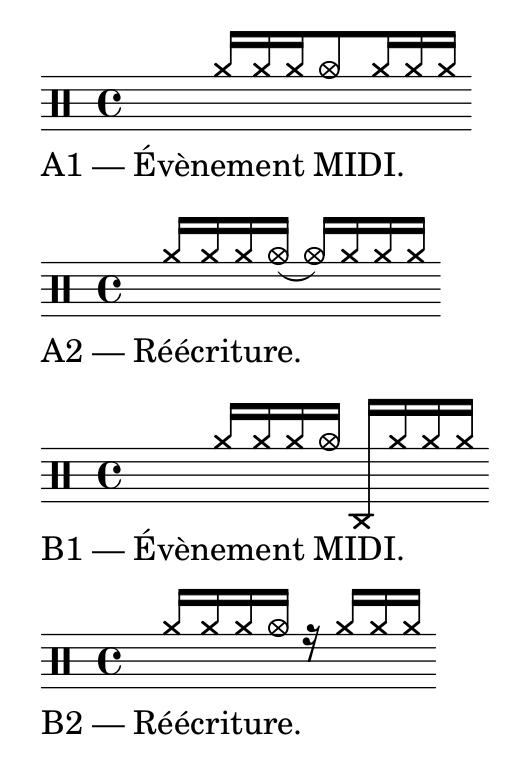
\includegraphics[height=80mm, width=60mm]{z_images/notation/reecriture/exemples_charley_1.png}\\\\

\textbf{Exemples à écrire en arbre :}\\
\begin{itemize}
	\item 
	SI (pas pf) ET (note sur un temps suivie de note en l’air) :\\
	$\Rightarrow$ (Temps1 : Note pertinente) + (Temps2 : Silence pertinent + Note pertinente.)\\
	\item
	Si (po ou co) déborde sur le temps suivant :\\
	$\Rightarrow$ Liaison car marchera dans tous les cas même la où le point ne marchera pas (voir A2).\\
	\item
	Une blanche sera écrite noir + soupir.\\\\
\end{itemize}
\subsubsection{Les régles de réécriture}
~~\\
\Tree[.$\frac{2}{8}$ [.x ][.tie ]]\Tree[.2/8 [.x ]]\\\\\\
\Tree[.1/4 [.x ][.tie ]]\Tree[.1/4 [.x ][.r ]]\\\\\\

\section{Conclusion}
Conclusion de ce chapitre.


%%%%%%%%%%%%%%%%%%%%%%%%%%%%%%%%%%%%%%%%%%%%%%%%%%%%%%%%%%%%%%%%
%% Deuxième partie

\part{Expérimentations}



%%%%%%%%%%%%%%%%%%%%%%%%%%%%%%%%%%%%%%%%%%%%%%%%%%%%%%
%% CORPUS
%%%%%%%%%%%%%%%%%%%%%%%%%%%%%%%%%%%%%%%%%%%%%%%%%%%%%%


\chapter{Corpus}
\label{chap:corpus}
\minitoc

\section{Introduction}
Dans ce chapitre...
\textbf{groove MIDI dataset}\\
	\url{https://magenta.tensorflow.org/datasets/groove}\\\\
	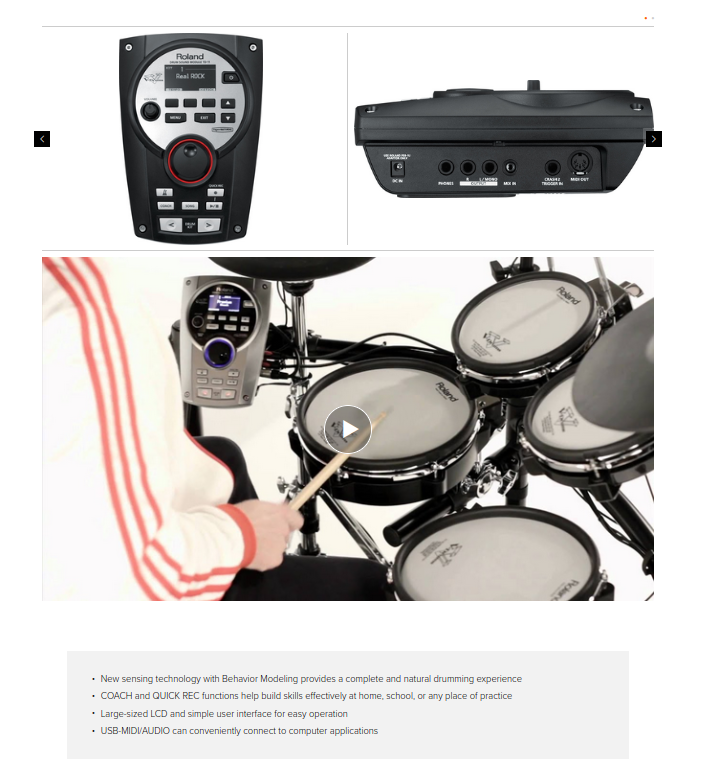
\includegraphics[height=60mm, width=60mm]{z_images/2_groove/roland_TD11.png}\\
	Des batteurs pro ont été engagés pour jouer sur un roland td-11\\\\
	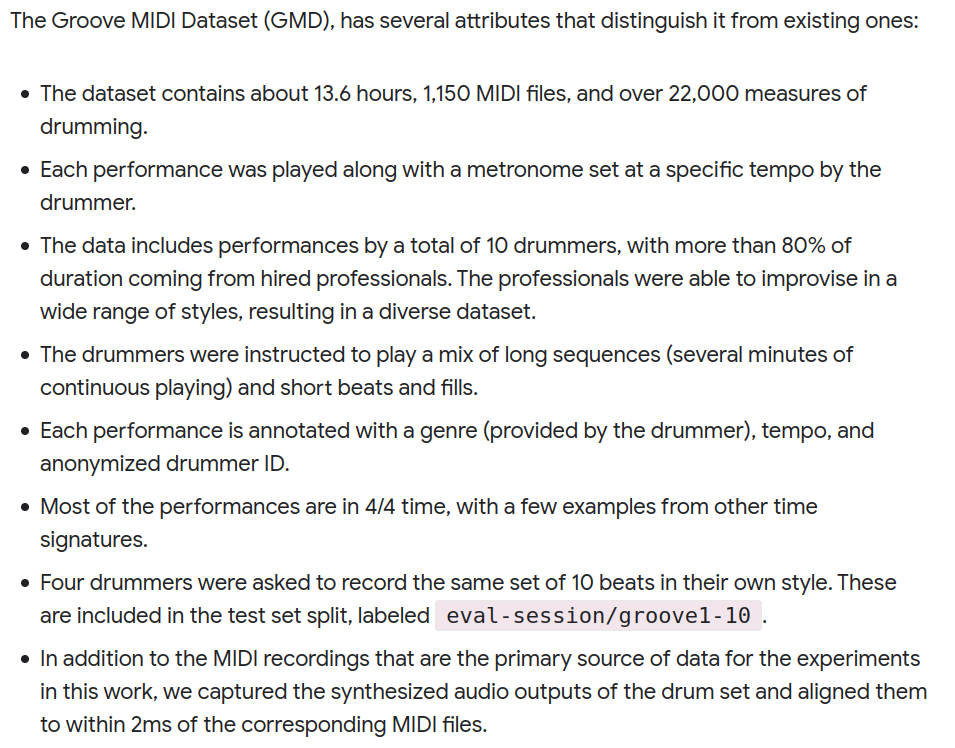
\includegraphics[height=80mm, width=110mm]{z_images/2_groove/dataset_how.png}\newpage{}
	\textbf{Les métadatas :}\\\\
	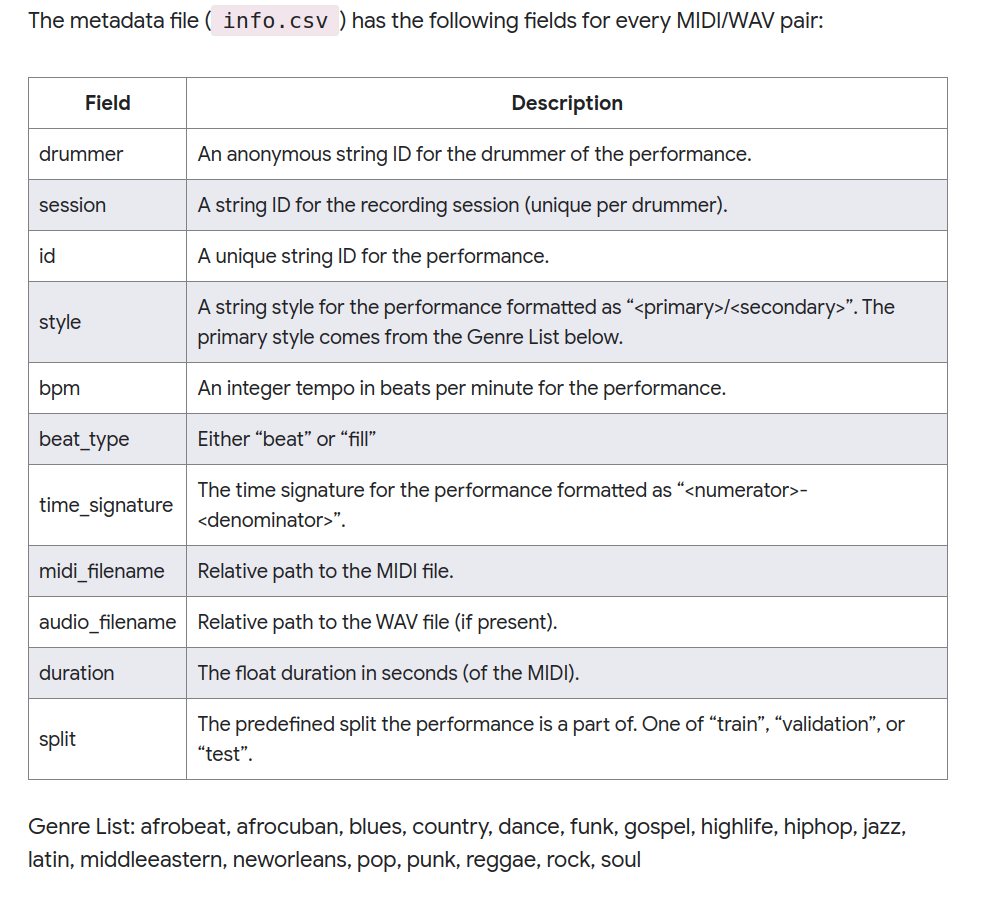
\includegraphics[height=85mm, 
	width=100mm]{z_images/2_groove/csv_metadata_struct.png}\\
	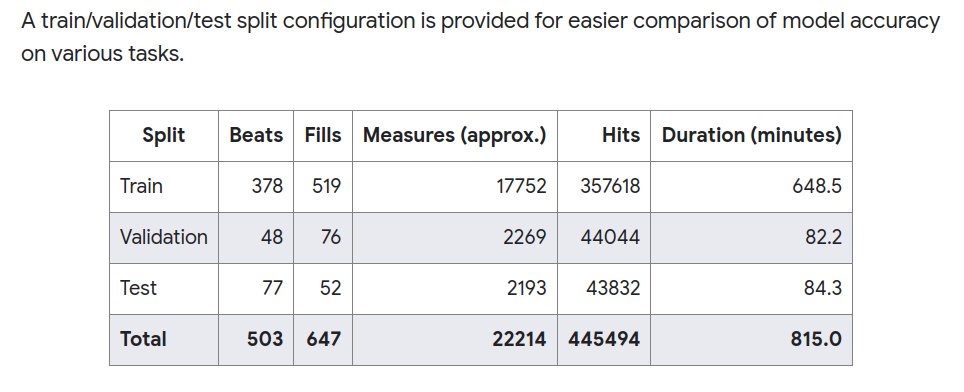
\includegraphics[height=50mm, width=120mm]{z_images/2_groove/train_validation_test.png}\\
	Détails (entre autres tensorflow avec le dataset) à :
	\url{https://magenta.tensorflow.org/datasets/groove#license}\\
	écouter le dataset groove
	\newpage
%Les transcriptions manuelles sont faites à partir des fichiers wav et celles de MuseScore à partir des fichiers MIDI.\\
\section{Partitions entières}
Mettre ici des partitions entièrement transcrites.
\section{Comparaisons de transcriptions}
\subsection*{0. Prise en main}
Pour la prise en main, les transcriptions manuelles ont été faites avec musescore au lieu de lilypond.
\textbf{Premiers tests sur drummer\_01/session3}\\

\textbf{\textit{Exemple 1 : 10\_rock-folk\_90\_beat\_4-4}}\\\\
\textbf{manuelle}\\
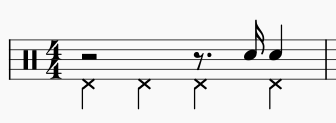
\includegraphics[height=25mm, width=70mm]{images/transcriptions_manuelles/0_prise_en_main/0_tests_drummer_01__session3/manuel_0.png} \\
\textbf{musescore}\\
\includegraphics[height=25mm, width=70mm]{images/transcriptions_manuelles/0_prise_en_main/0_tests_drummer_01__session3/musescore_0.png} \\
\begin{itemize}
	\item Erreur d’indication de mesure ;
	\item Mauvaise transcription d’une noire.\\
\end{itemize}
La noire du 4ème temps se retrouve sur le premier temps de la mesure suivante et elle se transforme en un triolet de double croches dont seules les deux premières seraient jouées.\\\\
\textbf{\textit{Exemple 2 : 10\_rock-folk\_90\_beat\_4-4}}\\\\
\textbf{manuelle}\\
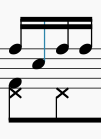
\includegraphics[height=30mm, width=25mm]{images/transcriptions_manuelles/0_prise_en_main/0_tests_drummer_01__session3/manuel_1.png} \\
\textbf{musescore}\\
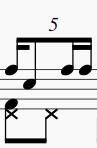
\includegraphics[height=30mm, width=25mm]{images/transcriptions_manuelles/0_prise_en_main/0_tests_drummer_01__session3/musescore_1.png} \\
\begin{itemize}
	\item Erreur de quantification : les doubles croches ont été interprétées en quintolet;\\
\end{itemize}
\textbf{\textit{Exemple 3 : 2\_jazz-swing\_185\_beat\_4-4}}
\\\\
\textbf{manuelle}\\
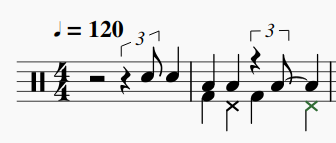
\includegraphics[height=30mm, width=65mm]{images/transcriptions_manuelles/0_prise_en_main/0_tests_drummer_01__session3/manuel_2.png} \\
\textbf{musescore}\\
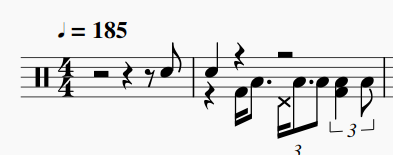
\includegraphics[height=30mm, width=65mm]{images/transcriptions_manuelles/0_prise_en_main/0_tests_drummer_01__session3/musescore_2.png} \\
\begin{itemize}
	\item L’indication de mesure est correcte mais tout a été décalé d’un temps car la première noire sur la caisse claire est jouée sur le 4ème temps et non sur le premier temps de la deuxième mesure comme l’indique la transcription de musescore.
	\item Les toms basses des 1er et 2ème temps de la mesure musescore auraient dû être sur les temps et non décalés d’une double croche vers la droite.\\
\end{itemize}
\textbf{Solutions aux pb rencontrés}\\\\
Existe-t-il un moyen de rectifier les erreurs d’indication de mesure et de décalage de temps des partitions MuseScores.\\
\begin{itemize}
	\item Changer dans manuellement dans MuseScore l’indication de mesure\footnote{\url{https://musescore.org/fr/manuel/indications-de-mesure}} fonctionne avec la transcription du MIDI. \\\\ 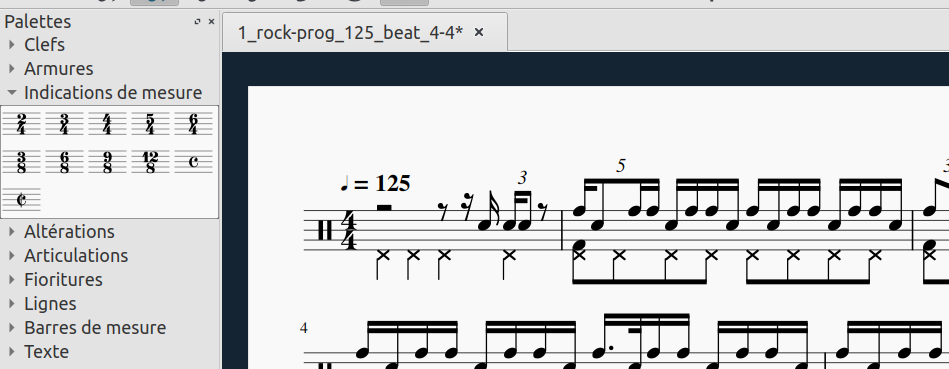
\includegraphics[height=30mm, width=65mm]{images/transcriptions_manuelles/0_prise_en_main/0_tests_drummer_01__session3/solution_0.png} \\
	\item Pour décaler tout d’un temps, on peut sélectionner les mesures en question en cliquant sur la première note de la séquence et en maj-cliquant sur la dernière, puis Ctrl-X Ctrl-V pour replacer le tout au bon endroit.\footnote{\url{https://musescore.org/fr/node/276292}}\\
\end{itemize}

\textit{À partir de la prochaine section, les indications de mesures erronées ou les décalages de temps qui ont des répercussions sur l’ensemble de la partition seront corrigés avant l’analyse.}\\\\
\textbf{Seconds tests sur drummer\_01/session1}\\\\
\textbf{\textit{Exemple 1 : 1\_funk\_80\_beat\_4-4}}
\textbf{manuelle}\\
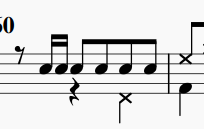
\includegraphics[height=25mm, width=40mm]{images/transcriptions_manuelles/0_prise_en_main/1_drummer_01__session1/Manuelle_0.png} \\
\textbf{musescore}\\
\includegraphics[height=25mm, width=40mm]{images/transcriptions_manuelles/0_prise_en_main/1_drummer_01__session1/musescore_0.png} \\
\begin{itemize}
	\item On dirait que lorsque certaines notes sont proches, elles se resserrent et suppriment celles qui aurait dû être sur le temps.\\
\end{itemize}
\textbf{\textit{Exemple 2 : 1\_funk\_80\_beat\_4-4}}
1\_funk\_80\_beat\_4-4\\\\
\textbf{manuelle}\\
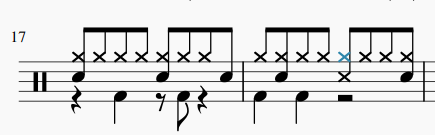
\includegraphics[height=25mm, width=70mm]{images/transcriptions_manuelles/0_prise_en_main/1_drummer_01__session1/Manuelle_1.png} \\
\textbf{musescore}\\
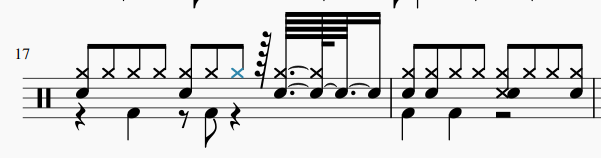
\includegraphics[height=25mm, width=70mm]{images/transcriptions_manuelles/0_prise_en_main/1_drummer_01__session1/MuseScore_1.png} \\
\begin{itemize}
	\item La caisse claire de la 2ème croche du 4ème temps de la 1ère mesure se transforme en une combinaison de quadruple/quintuple/double croches liées qui commence par un soupir et finit en débordant sur le premier temps de la mesure suivante. 
\end{itemize}
\newpage
\subsection*{1. Transcription des flas}
À partir de maintenant, les transcriptions manuelles seront faites avec LilyPond.
\subsubsection{Sur la question des flas}
Des exemples de notation flas tom/caisse-claire existent dans des partitions récentes (rythmique binaire J.-F. Juskowiak).\\
$\Rightarrow$ Ils faudra donc les prendre en compte dans les comparaisons de transcriptions.
De gauche à droite : transcription musescore, transcription manuelle.\\
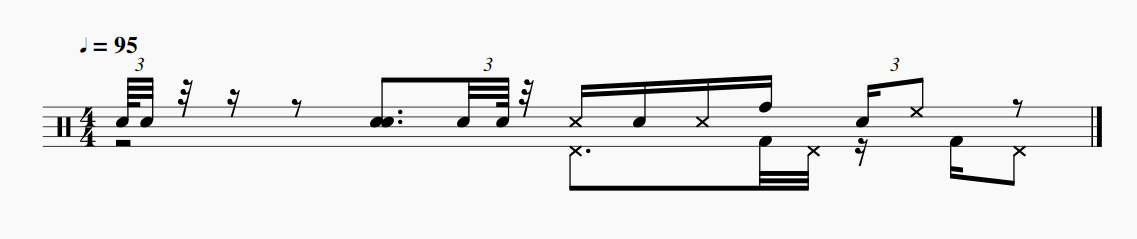
\includegraphics[height=20mm, width=80mm]{images/transcriptions_manuelles/1_transcriptions_flas/124_funk_95_fill_4-4_0.png}
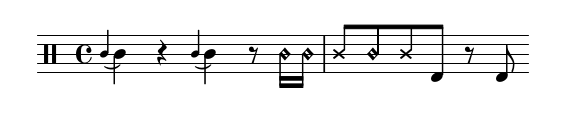
\includegraphics[height=20mm, width=80mm]{images/transcriptions_manuelles/1_transcriptions_flas/124_funk_95_fill_4-4_1.png}\\
Il manque des charley, je dois trouver comment faire des accords avec des têtes de notes différentes.\\\\
\subsection*{2. Autres}
- Chercher des exemples de silences, tuplets.\\
- Faire les observations avec des notations plus ou moins chargées.

\section{Contenu}
\subsection{Expérience 1 - 4/4 binaire}
\subsubsection{Partition de référence pour l’ouput}
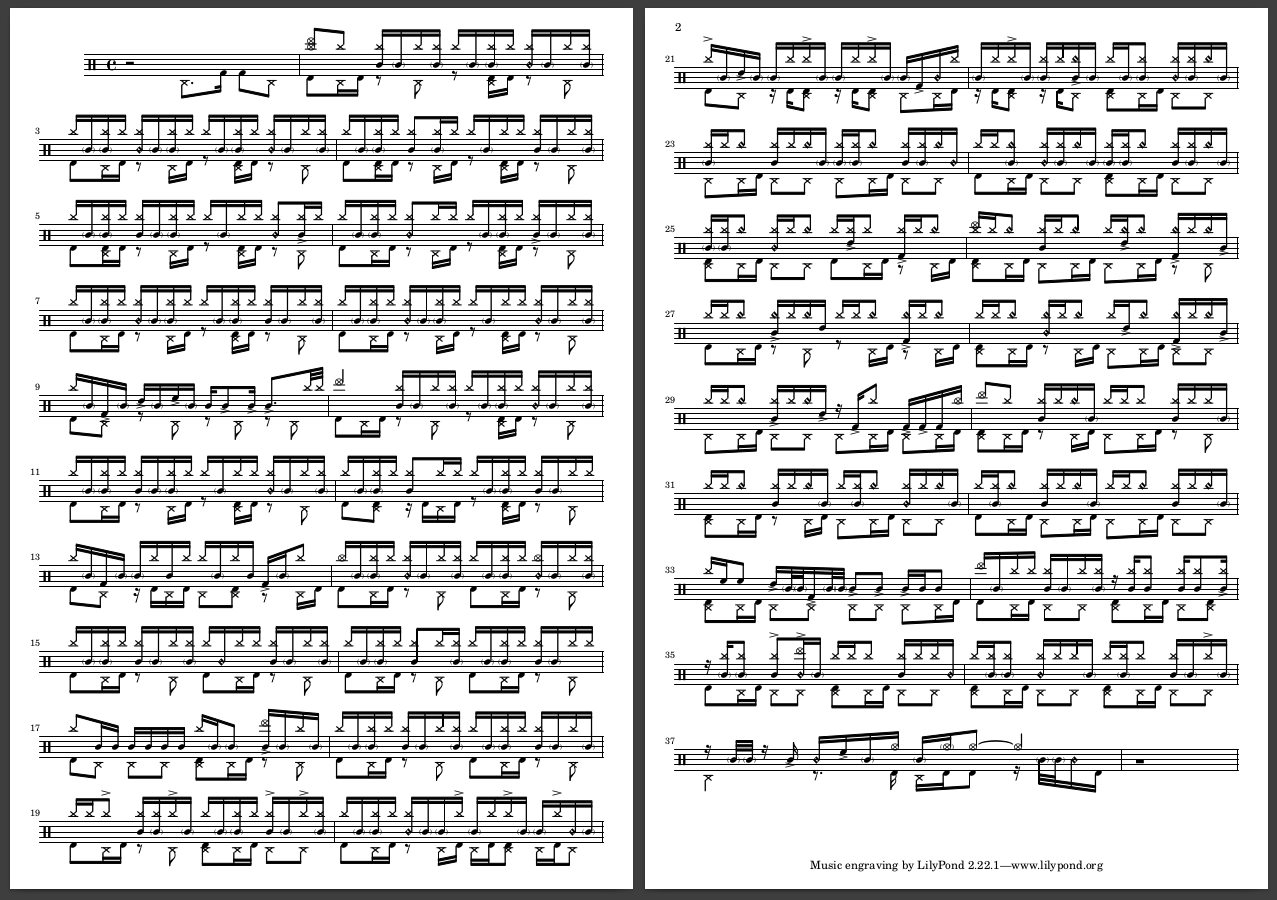
\includegraphics[height=120mm, width=160mm]{z_images/3_experimentations/experience_1/partition.png}
\subsubsection{Systèmes recherchés}
Textes :\\\\
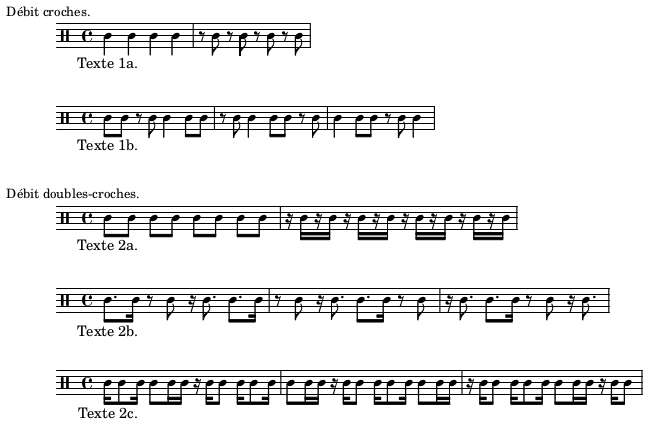
\includegraphics[height=70mm, width=95mm]{z_images/1_description_notation/systemes/0_textes_4-4_binaires.png}\\
Motifs :\\\\
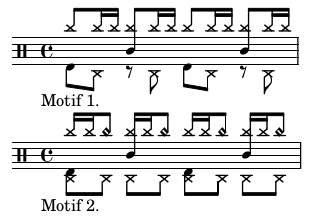
\includegraphics[height=30mm, width=40mm]{z_images/1_description_notation/systemes/1_motifs_4-4_binaires.png}\\\\
Systèmes résultants :\\\\
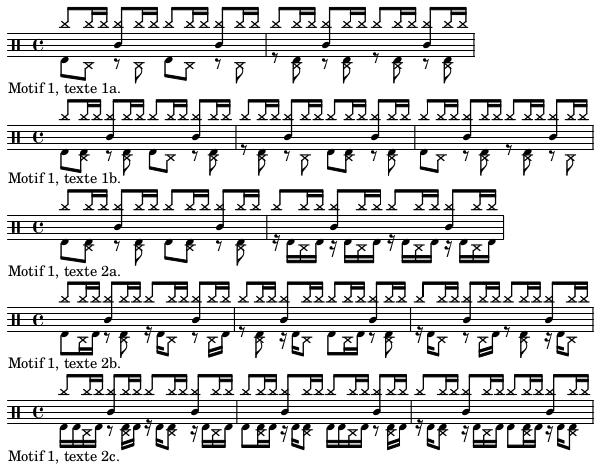
\includegraphics[height=75mm, width=85mm]{z_images/3_experimentations/experience_1/systeme_recherche_1.png}
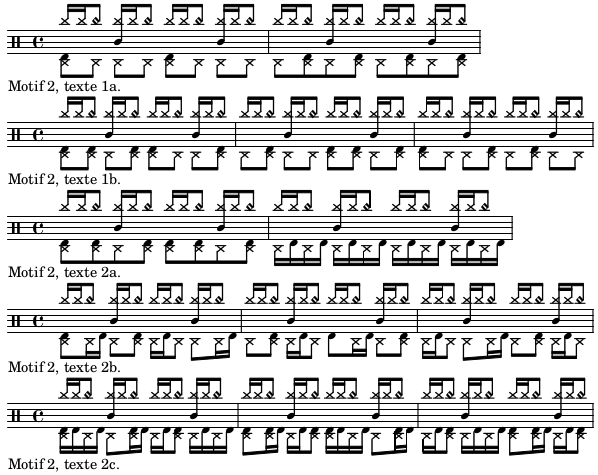
\includegraphics[height=75mm, width=85mm]{z_images/3_experimentations/experience_1/systeme_recherche_2.png}


\subsubsection{Représentation des systèmes en arbres de rythmes}

\resizebox{500pt}{!} {
	\Tree[.Motif\ 1\ +\ Texte\ 1a
	[.Mesure\ 1
	[.Temps\ 1 [rd\\bd ][ [rd\\pf ][rd ]]]
	[.Temps\ 2 [rd\\cc ][ [rd\\pf ][rd ]]]
	[.Temps\ 3 [rd\\bd ][ [rd\\pf ][rd ]]]
	[.Temps\ 4 [rd\\cc ][ [rd\\pf ][rd ]]] ]
	[.Mesure\ 2
	[.Temps\ 1 [rd ][ [rd\\bd\\pf ][rd ]]]
	[.Temps\ 2 [rd\\cc ][ [rd\\bd\\pf ][rd ]]]
	[.Temps\ 3 [rd ][ [rd\\bd\\pf ][rd ]]]
	[.Temps\ 4 [rd\\cc ][ [rd\\bd\\pf ][rd ]]] ]]}\\

\resizebox{500pt}{!} {
	\Tree[.Motif\ 1\ +\ Texte\ 1b
	[.Mesure\ 1
	[.Temps\ 1 [rd\\bd ][ [rd\\bd\\pf ][rd ]]]
	[.Temps\ 2 [rd\\cc ][ [rd\\bd\\pf ][rd ]]]
	[.Temps\ 3 [rd\\bd ][ [rd\\pf ][rd ]]]
	[.Temps\ 4 [rd\\cc ][ [rd\\bd\\pf ][rd ]]] ]
	[.Mesure\ 2
	[.Temps\ 1 [rd ][ [rd\\bd\\pf ][rd ]]]
	[.Temps\ 2 [rd\\cc ][ [rd\\pf ][rd ]]]
	[.Temps\ 3 [rd\\bd ][ [rd\\bd\\pf ][rd ]]]
	[.Temps\ 4 [rd\\cc ][ [rd\\bd\\pf ][rd ]]] ]
	[.Mesure\ 3
	[.Temps\ 1 [rd\\bd ][ [rd\\pf ][rd ]]]
	[.Temps\ 2 [rd\\cc ][ [rd\\bd\\pf ][rd ]]]
	[.Temps\ 3 [rd ][ [rd\\bd\\pf ][rd ]]]
	[.Temps\ 4 [rd\\cc ][ [rd\\pf ][rd ]]] ]]}\\

\resizebox{500pt}{!} {
	\Tree[.Motif\ 1\ +\ Texte\ 2a
	[.Mesure\ 1
	[.Temps\ 1 [rd\\bd ][ [rd\\bd\\pf ][rd ]]]
	[.Temps\ 2 [rd\\cc ][ [rd\\bd\\pf ][rd ]]]
	[.Temps\ 3 [rd\\bd ][ [rd\\bd\\pf ][rd ]]]
	[.Temps\ 4 [rd\\cc ][ [rd\\bd\\pf ][rd ]]] ]
	[.Mesure\ 2
	[.Temps\ 1 [rd ][bd ][rd\\pf ][rd\\bd ]]
	[.Temps\ 2 [rd\\cc ][bd ][rd\\pf ][rd\\bd ]]
	[.Temps\ 3 [rd ][bd ][rd\\pf ][rd\\bd ]]
	[.Temps\ 4 [rd\\cc ][bd ][rd\\pf ][rd\\bd ]] ]]}\\

\resizebox{500pt}{!} {
	\Tree[.Motif\ 1\ +\ Texte\ 2b
	[.Mesure\ 1
	[.Temps\ 1 [rd\\bd ][ [rd\\pf ][rd\\bd ]]]
	[.Temps\ 2 [rd\\cc ][ [rd\\bd\\pf ][rd ]]]
	[.Temps\ 3 [rd ][bd ][rd\\pf ][rd ]]
	[.Temps\ 4 [rd\\cc ][ [rd\\pf ][rd\\bd ]]] ]
	[.Mesure\ 2
	[.Temps\ 1 [rd\\ ][ [rd\\bd\\pf ][rd ]]]
	[.Temps\ 2 [rd\\cc ][bd ][rd\\pf ][rd ]]
	[.Temps\ 3 [rd\\bd ][ [rd\\pf ][rd\\bd ]]]
	[.Temps\ 4 [rd\\cc ][ [rd\\bd\\pf ][rd ]]] ]
	[.Mesure\ 3
	[.Temps\ 1 [rd ][bd ][rd\\pf ][rd ]]
	[.Temps\ 2 [rd\\cc ][ [rd\\pf ][rd\\bd ]]]
	[.Temps\ 3 [rd ][ [rd\\bd\\pf ][rd ]]]
	[.Temps\ 4 [rd\\cc ][bd ][rd\\pf ][rd ]]] ] }\\

\resizebox{500pt}{!} {
	\Tree[.Motif\ 1\ +\ Texte\ 2c
	[.Mesure\ 1
	[.Temps\ 1 [rd\\bd ][bd ][rd\\pf ][rd\\bd ]]
	[.Temps\ 2 [rd\\cc ][ [rd\\bd\\pf ][rd\\bd ]]]
	[.Temps\ 3 [rd ][bd ][rd\\bd\\pf ][rd ]]
	[.Temps\ 4 [rd\\cc ][bd ][rd\\pf ][rd\\bd ]] ]
	[.Mesure\ 2
	[.Temps\ 1 [rd\\bd ][ [rd\\bd\\pf ][rd\\bd ]]]
	[.Temps\ 2 [rd\\cc ][bd ][rd\\bd\\pf ][rd ]]
	[.Temps\ 3 [rd\\bd ][bd ][rd\\pf ][rd\\bd ]]
	[.Temps\ 4 [rd\\cc ][ [rd\\bd\\pf ][rd\\bd ]]] ]
	[.Mesure\ 3
	[.Temps\ 1 [rd ][bd ][rd\\bd\\pf ][rd ]]
	[.Temps\ 2 [rd\\cc ][bd ][rd\\pf ][rd\\bd ]]
	[.Temps\ 3 [rd\\bd ][ [rd\\bd\\pf ][rd\\bd ]]]
	[.Temps\ 4 [rd\\cc ][bd ][rd\\bd\\pf ][rd ]]] ] }\\\\

\subsubsection{Séparation des voix}
Motif\ 1\ +\ Texte\ 1a\\\\
\textit{Voix haute}\\
\resizebox{500pt}{!} {
	\Tree[.Motif\ 1\ +\ Texte\ 1a
	[.Mesure\ 1
	[.Temps\ 1 [rd ][ [rd ][rd ]]]
	[.Temps\ 2 [rd\\cc ][ [rd ][rd ]]]
	[.Temps\ 3 [rd ][ [rd ][rd ]]]
	[.Temps\ 4 [rd\\cc ][ [rd ][rd ]]] ]
	[.Mesure\ 2
	[.Temps\ 1 [rd ][ [rd ][rd ]]]
	[.Temps\ 2 [rd\\cc ][ [rd ][rd ]]]
	[.Temps\ 3 [rd ][ [rd ][rd ]]]
	[.Temps\ 4 [rd\\cc ][ [rd ][rd ]]] ]]}\\

\textit{Voix basse}\\
\resizebox{500pt}{!} {
	\Tree[.Motif\ 1\ +\ Texte\ 1a
	[.Mesure\ 1
	[.Temps\ 1 [bd ][ [pf ][t ]]]
	[.Temps\ 2 [t ][ [pf ][t ]]]
	[.Temps\ 3 [bd ][ [pf ][t ]]]
	[.Temps\ 4 [t ][ [pf ][t ]]] ]
	[.Mesure\ 2
	[.Temps\ 1 [t ][ [bd\\pf ][t ]]]
	[.Temps\ 2 [t ][ [bd\\pf ][t ]]]
	[.Temps\ 3 [t ][ [bd\\pf ][t ]]]
	[.Temps\ 4 [t ][ [bd\\pf ][t ]]] ]]}\\

Motif\ 1\ +\ Texte\ 1b\\\\
\textit{Voix haute}\\
\resizebox{500pt}{!} {
	\Tree[.Motif\ 1\ +\ Texte\ 1b
	[.Mesure\ 1
	[.Temps\ 1 [rd ][ [rd ][rd ]]]
	[.Temps\ 2 [rd\\cc ][ [rd ][rd ]]]
	[.Temps\ 3 [rd ][ [rd ][rd ]]]
	[.Temps\ 4 [rd\\cc ][ [rd ][rd ]]] ]
	[.Mesure\ 2
	[.Temps\ 1 [rd ][ [rd ][rd ]]]
	[.Temps\ 2 [rd\\cc ][ [rd ][rd ]]]
	[.Temps\ 3 [rd ][ [rd ][rd ]]]
	[.Temps\ 4 [rd\\cc ][ [rd ][rd ]]] ]
	[.Mesure\ 3
	[.Temps\ 1 [rd ][ [rd ][rd ]]]
	[.Temps\ 2 [rd\\cc ][ [rd ][rd ]]]
	[.Temps\ 3 [rd ][ [rd ][rd ]]]
	[.Temps\ 4 [rd\\cc ][ [rd ][rd ]]] ]]}\\

\textit{Voix basse}\\
\resizebox{500pt}{!} {
	\Tree[.Motif\ 1\ +\ Texte\ 1b
	[.Mesure\ 1
	[.Temps\ 1 [bd ][ [bd\\pf ][t ]]]
	[.Temps\ 2 [t ][ [bd\\pf ][t ]]]
	[.Temps\ 3 [bd ][ [pf ][t ]]]
	[.Temps\ 4 [t ][ [bd\\pf ][t ]]] ]
	[.Mesure\ 2
	[.Temps\ 1 [t ][ [bd\\pf ][t ]]]
	[.Temps\ 2 [t ][ [pf ][t ]]]
	[.Temps\ 3 [bd ][ [bd\\pf ][t ]]]
	[.Temps\ 4 [t ][ [bd\\pf ][t ]]] ]
	[.Mesure\ 3
	[.Temps\ 1 [bd ][ [pf ][t ]]]
	[.Temps\ 2 [t ][ [bd\\pf ][t ]]]
	[.Temps\ 3 [t ][ [bd\\pf ][t ]]]
	[.Temps\ 4 [t ][ [pf ][t ]]] ]]}\\

Motif\ 1\ +\ Texte\ 2a\\\\
\textit{Voix haute}\\
\resizebox{500pt}{!} {
	\Tree[.Motif\ 1\ +\ Texte\ 2a
	[.Mesure\ 1
	[.Temps\ 1 [rd ][ [rd ][rd ]]]
	[.Temps\ 2 [rd\\cc ][ [rd ][rd ]]]
	[.Temps\ 3 [rd ][ [rd ][rd ]]]
	[.Temps\ 4 [rd\\cc ][ [rd ][rd ]]] ]
	[.Mesure\ 2
	[.Temps\ 1 [rd ][t ][rd ][rd ]]
	[.Temps\ 2 [rd\\cc ][t ][rd ][rd ]]
	[.Temps\ 3 [rd ][t ][rd ][rd ]]
	[.Temps\ 4 [rd\\cc ][t ][rd ][rd ]] ]]}\\

\textit{Voix basse}\\
\resizebox{500pt}{!} {
	\Tree[.Motif\ 1\ +\ Texte\ 2a
	[.Mesure\ 1
	[.Temps\ 1 [bd ][ [bd\\pf ][t ]]]
	[.Temps\ 2 [t ][ [bd\\pf ][t ]]]
	[.Temps\ 3 [bd ][ [bd\\pf ][t ]]]
	[.Temps\ 4 [t ][ [bd\\pf ][t ]]] ]
	[.Mesure\ 2
	[.Temps\ 1 [t ][bd ][pf ][bd ]]
	[.Temps\ 2 [t ][bd ][pf ][bd ]]
	[.Temps\ 3 [t ][bd ][pf ][bd ]]
	[.Temps\ 4 [t ][bd ][pf ][bd ]] ]]}\\

Motif\ 1\ +\ Texte\ 2b\\\\
\textit{Voix haute}\\
\resizebox{500pt}{!} {
	\Tree[.Motif\ 1\ +\ Texte\ 2b
	[.Mesure\ 1
	[.Temps\ 1 [rd ][ [rd ][rd ]]]
	[.Temps\ 2 [rd\\cc ][ [rd ][rd ]]]
	[.Temps\ 3 [rd ][t ][rd ][rd ]]
	[.Temps\ 4 [rd\\cc ][ [rd ][rd ]]] ]
	[.Mesure\ 2
	[.Temps\ 1 [rd\\ ][ [rd ][rd ]]]
	[.Temps\ 2 [rd\\cc ][t ][rd ][rd ]]
	[.Temps\ 3 [rd ][ [rd ][rd ]]]
	[.Temps\ 4 [rd\\cc ][ [rd ][rd ]]] ]
	[.Mesure\ 3
	[.Temps\ 1 [rd ][t ][rd ][rd ]]
	[.Temps\ 2 [rd\\cc ][ [rd ][rd ]]]
	[.Temps\ 3 [rd ][ [rd ][rd ]]]
	[.Temps\ 4 [rd\\cc ][t ][rd ][rd ]]] ] }\\

\textit{Voix basse}\\
\resizebox{500pt}{!} {
	\Tree[.Motif\ 1\ +\ Texte\ 2b
	[.Mesure\ 1
	[.Temps\ 1 [bd ][ [pf ][bd ]]]
	[.Temps\ 2 [t ][ [bd\\pf ][t ]]]
	[.Temps\ 3 [t ][bd ][pf ][t ]]
	[.Temps\ 4 [t ][ [pf ][bd ]]] ]
	[.Mesure\ 2
	[.Temps\ 1 [t ][ [bd\\pf ][t ]]]
	[.Temps\ 2 [t ][bd ][pf ][t ]]
	[.Temps\ 3 [bd ][ [pf ][bd ]]]
	[.Temps\ 4 [t ][ [bd\\pf ][t ]]] ]
	[.Mesure\ 3
	[.Temps\ 1 [t ][bd ][pf ][t ]]
	[.Temps\ 2 [t ][ [pf ][bd ]]]
	[.Temps\ 3 [t ][ [bd\\pf ][t ]]]
	[.Temps\ 4 [t ][bd ][pf ][t ]]] ] }\\\\

Motif\ 1\ +\ Texte\ 2c\\\\
\textit{Voix haute}\\
\resizebox{500pt}{!} {
	\Tree[.Motif\ 1\ +\ Texte\ 2c
	[.Mesure\ 1
	[.Temps\ 1 [rd ][t ][rd ][rd ]]
	[.Temps\ 2 [rd\\cc ][ [rd ][rd ]]]
	[.Temps\ 3 [rd ][t ][rd ][rd ]]
	[.Temps\ 4 [rd\\cc ][t ][rd ][rd ]] ]
	[.Mesure\ 2
	[.Temps\ 1 [rd ][ [rd ][rd ]]]
	[.Temps\ 2 [rd\\cc ][t ][rd ][rd ]]
	[.Temps\ 3 [rd ][t ][rd ][rd ]]
	[.Temps\ 4 [rd\\cc ][ [rd ][rd ]]] ]
	[.Mesure\ 3
	[.Temps\ 1 [rd ][t ][rd ][rd ]]
	[.Temps\ 2 [rd\\cc ][t ][rd ][rd ]]
	[.Temps\ 3 [rd ][ [rd ][rd ]]]
	[.Temps\ 4 [rd\\cc ][t ][rd ][rd ]]] ] }\\\\

\textit{Voix basse}\\
\resizebox{500pt}{!} {
	\Tree[.Motif\ 1\ +\ Texte\ 2c
	[.Mesure\ 1
	[.Temps\ 1 [bd ][bd ][pf ][bd ]]
	[.Temps\ 2 [t ][ [bd\\pf ][bd ]]]
	[.Temps\ 3 [t ][bd ][bd\\pf ][t ]]
	[.Temps\ 4 [t ][bd ][pf ][bd ]] ]
	[.Mesure\ 2
	[.Temps\ 1 [bd ][ [bd\\pf ][bd ]]]
	[.Temps\ 2 [t ][bd ][bd\\pf ][t ]]
	[.Temps\ 3 [bd ][bd ][pf ][bd ]]
	[.Temps\ 4 [t ][ [bd\\pf ][bd ]]] ]
	[.Mesure\ 3
	[.Temps\ 1 [t ][bd ][bd\\pf ][t ]]
	[.Temps\ 2 [t ][bd ][pf ][bd ]]
	[.Temps\ 3 [bd ][ [bd\\pf ][bd ]]]
	[.Temps\ 4 [t ][bd ][bd\\pf ][t ]]] ] }\\\\
\newpage


\subsubsection{Règles de réécriture pour le 4/4 binaire}

\resizebox{70pt}{!} {
	\Tree[.1/4 [t ][x ][x ][x ] ]
}\ \ \ \ \ $\Rightarrow$\ \ \ \ \
\resizebox{70pt}{!} {
	\Tree[.1/4 [r ][x ][x ][x ] ]
}\\\\

\resizebox{70pt}{!} {
	\Tree[.1/4 [x ][t ][x ][x ]]
}\ \ \ \ \ $\Rightarrow$\ \ \ \ \
\resizebox{50pt}{!} {
	\Tree[.1/4 [x ][ [x ][x ]]]
}\\\\

\resizebox{70pt}{!} {
	\Tree[.1/4 [t ][x ][x ][t ] ]
}\ \ \ \ \ $\Rightarrow$\ \ \ \ \
\resizebox{50pt}{!} {
	\Tree[.1/4 [ [r ][x ]][x ] ]
}\\\\

\resizebox{50pt}{!} {
	\Tree[.1/4 [t ][ [x ][x ]]]
}\ \ \ \ \ $\Rightarrow$\ \ \ \ \
\resizebox{50pt}{!} {
	\Tree[.1/4 [r ][ [x ][x ]]]
}\\\\

\resizebox{50pt}{!} {
	\Tree[.1/4 [t ][ [x ][t ]] ]
}\ \ \ \ \ $\Rightarrow$\ \ \ \ \
\resizebox{30pt}{!} {
	\Tree[.1/4 [r ][x ] ]
}\\\\

\resizebox{50pt}{!} {
	\Tree[.1/4 [x ][ [x ][t ]] ]
}\ \ \ \ \ $\Rightarrow$\ \ \ \ \
\resizebox{30pt}{!} {
	\Tree[.1/4 [x ][x ] ]
}
\newpage

\subsection{Expérience 2}
\subsubsection{Partition de référence pour l’ouput}
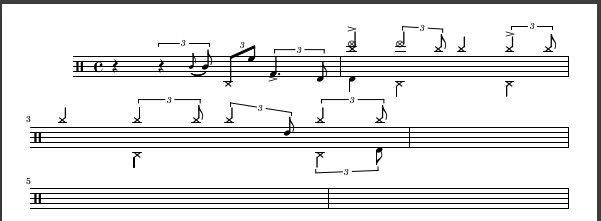
\includegraphics[height=50mm, width=160mm]{z_images/3_experimentations/experience_2/partition.png}\\\\
\textit{En cours…}
\newpage
\subsection{squant : parsing du fichier midi}
squant lit le midi\\
grammaire wta qui détermine le poid\\
La distance est automatiquement déterminée par squant\\
distance à l’input\\
complexité de la notation

On veut minimiser le coût et la distance $\Rightarrow$ Trouver un compromis.

./build/squant2 -h

Essayer le lire un fichier midi avec squant2
lire mesure par mesure
Regarder les wta(grammaire)

\subsubsection{Quelques tests de lecture midi}
\begin{verbatim}
Les 4 messages suivants sont présents dans tous les tests qui suivent :
[ info] schema file: test/schema/schema-01.wta (??? weight model option)
[warning] no declaration MAX\_GRACE in grammar file test/schema/schema-01.wta
[warning] no declaration TIMESIG in grammar file test/schema/schema-01.wta
[warning] MIDIfile has not joined tracks

./build/squant2 -v 4 -a test/schema/schema-01.wta -m 004_jazz-funk_116_beat_4-4.mid -config ./params.ini
[error] at least one of the options -bars or -barsec mandatory

./build/squant2 -verbosity 4 -schema test/schema/schema-01.wta -midi 004\_jazz-funk\_116\_beat\_4-4.mid -config ./params.ini -barsec 3

squant2: /home/martin/qparselib/src/schemata/SymbLabel.cpp:44: static label_t SymbLabel::make(unsigned char, SymbLabel::Kind, short unsigned int, short unsigned int): Assertion `info2 < 512' failed.
Abandon (core dumped)
\end{verbatim}

Tester squant2 avec le fichiers midi du corpus du gitlab\\\\

La commande suivante :
\begin{verbatim}
	build/squant2 -v 5 -a ./test/schema/schema-03-R.wta -m ~/corpus-master_qparselib/103-SaintSaens-elephant/perf/103_FJ.mid -config ./params.ini -mono -barsec 3.0 -ts 3/4	
\end{verbatim}

Donne :\\
(1) 3($\bullet$, $\overline{2}$:2($\bullet$, ), )\\
(2) 3($\bullet$, $\overline{2}$:2($\bullet$, $\bullet$), )\\
(3) 3($\bullet$, $\overline{2}$:2($\bullet$, $\circ$), )\\\\

% Reste de l’arbre avec des caractères pas encore fonctionnels :
%(4) 3(2̅(2̅(2̅(●, ●), ⏑), ⏑), ⏑:2, )
%(5) 3(2̅(2̅(●, ○), ●), ●:2, )
%(6) 3(2̅(●, 2̅(●, 2̅(○, ●))), ⏑:2, )
%(7) 3(2̅(●, ●), ●:2, )
%(8) 3(2̅(●, 2̅(●, 2̅(⏑, ●))), 2̅(⏑, 2̅(●, ○)), ●)
%(9) 3(●, ●:2, )
%(10) 3(●, 2̅:2(●, 2̅(●, 2̅(⏑, ●))), )
%(11) 3(⏑, 2̅:2(●, ○), )
%(12) 3(●, ⏑, ●)
%(13) 3(●, 2̅:2(2̅(●, 2̅(○, ●)), 2̅(⏑, 2̅(○, ●))), )
%(14) 3(⏑, 2̅:2(●, 2̅(●, ○)), )
%(15) 3(●, ●:2, )
%(16) 3(●, ○:2, )

Pour comprendre les grammaires :\\
Regarder les fichiers wta commentés.\\
https://qparse.gitlabpages.inria.fr/docs/scientific/\\
A\_Parse-based\_Framework\_for\_Coupled\_RhythmQuantization\_and\_Score\_Structuring.pdf
Réfléchir au coût de notation (grace notes, etc.)
\newpage

\subsubsection{cluster.md}
%https://gitlab.inria.fr/qparse/qparselib/-/blob/distance/notes/clusters.md\\\\

\textbf{Caroms of input events}\\

Carom is a synonym for « pileup ». An alternative term could be « cluster » (in the Musical sense, not in the ML sense!).\\

----------------------------------------------------------\\

\textbf{input segment}\\

we assume given in input a sequence of MIDI events $e_0, \ldots, e_n$​​ called "input segment".\\

Every input event is $e_i$ is made of :
\begin{itemize}
	\item an `ON`/`OFF` flag
	\item a MIDI pitch value in $0..127$​
	\item a MIDI velocity value in $0..127$
	\item a date in Real Time Unit (RTU) = seconds, or equivalently MIDI ticks.\\
\end{itemize}

The input events are time-increasing:
$$ date(e_0) \leq  date(e_1) \leq \ldots \leq date(e_n)$$

\textbf{attention:} input event $\neq$​ note (in score):

One input event may have different roles wrt the output score:
\begin{itemize}
	\item begining of note
	\item grace note
	\item trill
	\item end of note
	\item rest
	\item just ignored.\\e.g. in general in MIDI drum input, the `OFF` events will be ignored, but not for piano input.\\
\end{itemize}

----------------------------------------------------------\\

\textbf{Parsing}\\

During parsing, we try several alignements of the input events to particular points in the timeline.\\
The points for alignement are defined by time division, according to a derivation (parse tree) for a CF grammar (actually a tree in a regular tree grammar language).\\

The temporal alignment of an event is done to the point that is the closest to the date of event.
This way, it may happen that several events are aligned to the same point.\\
\newpage

----------------------------------------------------------\\

\textbf{Carom}\\

A carom is a sequence $e_i,\ldots, e_{i+k}$​​ of successive input events (\textit{i.e} a subsequence of the input segment), that ought to be aligned to the same time point. In practice, it is defined by the input segment, $i$ and $k$.\\

Intuitively, it means that the corresponding notes (or rests) will be simultaneous in the output score (e.g. notes in chords, or in different polyphonic voices), or that they will be grace notes.\\

Formally, we define for every transcription case (monophonic instrument, drum, guitar, piano...) a function that depends on the that takes in input\\
\begin{itemize}
	\item a carom $C = e_i,\ldots, e_{i+k}$,
	\item an index $0 \leq j \leq k$,\\
\end{itemize}


and returns the \textit{role} the input event  $e_{i+j}$ in $C$, among:\\
\begin{itemize}
	\item `Ignored`,
	\item `Note`,
	\item `Rest`,
	\item `Staccato`,
	\item `GraceNote`,
	\item `GraceRest`,
	\item maybe more to come...\\
\end{itemize}

For instance, in the case of drum transcription, all `OFF` events are ignored.\\

\textbf{Example 1:}\\\\
In the case of \textbf{drum} transcription, all the pitchs of the following events correspond to the snare-drum (sd).

\begin{table}[h]
\centering
\begin{tabular}{|c|c|c|c|c|}\hline
	event & $e_1$ & $e_2$ & $e_3$ & $e_4$ \\ \hline
	flag & ON & OFF & ON & OFF \\
	pitch & 38 & 38 & 38 & 38 \\ \hline
\end{tabular}	
\end{table}

Therefore we have a sd "flam" (\url{https://en.wikipedia.org/wiki/Drum\_rudiment#Flam}), defined by the following roles:

\begin{table}[h]
	\centering
	\begin{tabular}{|c|c|c|c|c|}\hline
		event & $e_1$ & $e_2$ & $e_3$ & $e_4$ \\ \hline
		role  & GraceNote & Ignored & Note  & Ignored \\ \hline
	\end{tabular}	
\end{table}

We say that $e_3$ is the \textit{main note} associated to (or \textit{decorated by}) the grace note $e_1$.\\

When $e_{i+j}$​ is a grace note ('flam' in the case of drum), we assume moreover a second mapping, called \textit{main}, that associate to $j$​  the index in $[j+1, k]$​ of the corresponding main note.\\

Example 1': in the previous example, $main(1) = 3$.\\



\textbf{Example 2:}\\\\¨
In the case of **monophonic** transcription, the following events: 

| event | $e_1$ | $e_2$ | $e_3$ |
| :---: | :---: | :---: | :---: |
| flag  |  ON   |  OFF  |  ON   |
| pitch |  64   |  64   |  62   |

also correspond to a grace note followed by a note:



| event |   $e_1$   |  $e_2$  | $e_3$ |
| :---: | :-------: | :-----: | :---: |
| role  | GraceNote | Ignored | Note  |



Example 3: still in the case of **monophonic** transcription, for the following events: 

| event | $e_1$ | $e_2$ | $e_3$ |
| :---: | :---: | :---: | :---: |
| flag  |  ON   |  ON   |  OFF  |
| pitch |  64   |  62   |  64   |

we also have the same roles as in Ex.2:



| event |   $e_1$   | $e_2$ |  $e_3$  |
| :---: | :-------: | :---: | :-----: |
| role  | GraceNote | Note  | Ignored |

Indeed, we ignore that fact that the OFF $e_3$ happens  after the ON $e_2$ of next note (e.g. because of the end gesture of the player on the keyboard), because we are in the monophonic case. 



Note that here, we process directly the MIDI input. No pre-processing is assumed, e.g. for eliminating overlaps between the notes 64 and 62. Somehow, elimination of overlaps is ensured by the *role* function for the monophonic case.



Example 4: Back to the case of **drum** transcription, the pitch of $e_1$​​ and $e_2$​ below corresponds to a tom and the one of $e_3, e_4$​ to the sd.

|   event    | $e_1$ | $e_2$ | $e_3$ | $e_4$ |
| :--------: | :---: | :---: | :---: | :---: |
|    flag    |  ON   |  OFF  |  ON   |  OFF  |
|   pitch    |  48   |  48   |  38   |  38   |
| timestamps |  t\_1  |  t\_2  |  t\_3  |  t\_4  |

It could be interpreted either as two simultaneous tom and sd notes, or as a flam between the tom and the sd (the tom is the grace note, the sd the main note). We choose between the two cases according to the "On Tick" distance $t_3 - t_1$.
More precisely, we assume a threshold $\varepsilon$​ such that:

- if $t_3 - t_1 < \varepsilon$​​ then we have 2 simultaneous notes  ("polyphony", between tom and sd, written as a chord):

| event | $e_1$ |  $e_2$  | $e_3$ |  $e_4$  |
| :---: | :---: | :-----: | :---: | :-----: |
| role  | Note  | Ignored | Note  | Ignored |

- if $t_3 - t_1 ≥ \varepsilon$ then we have a flam between tom and sd (written as a grace note):

| event |   $e_1$   |  $e_2$  | $e_3$ |  $e_4$  |
| :---: | :-------: | :-----: | :---: | :-----: |
| role  | GraceNote | Ignored | Note  | Ignored |

The threshold $\varepsilon$ may depend on the latency of an electronic  (MIDI) drum kit used for recording, and/or neuro-acoustic features such as the duration between 2 percussive events above which the perception change from simultaneous, to the phoneme '*flam*'.


\subsubsection{Contributions}
Contribution sur la branch « distance » dans :\\
\begin{itemize}
	\item qparselib/notes/cluster.md
	\item qparselib/src/segment/import/ :\\
	      DrumCode hpp et cpp\\
\end{itemize}
\newpage
\section{Conclusion}
Conclusion de ce chapitre.


%%%%%%%%%%%%%%%%%%%%%%%%%%%%%%%%%%%%%%%%%%%%%%%%%%%%%%
%% RÉSULTATS
%%%%%%%%%%%%%%%%%%%%%%%%%%%%%%%%%%%%%%%%%%%%%%%%%%%%%%

\chapter{Résultats}
\label{chap:resultats}
\minitoc

\textit{\\Résultats (chapitre~\ref{chap:resultats})~: les résultats
obtenus sur chacune des expériences~;}

\section{Introduction}
Dans ce chapitre...

\section{Contenu}
Une section dans ce chapitre...

\section{Conclusion}
Conclusion de ce chapitre.


%%%%%%%%%%%%%%%%%%%%%%%%%%%%%%%%%%%%%%%%%%%%%%%%%%%%%%
%% DISCUSSION
%%%%%%%%%%%%%%%%%%%%%%%%%%%%%%%%%%%%%%%%%%%%%%%%%%%%%%

\chapter{Discussion}
\label{chap:discussion}
\minitoc

\textit{\\Discussion (chapitre~\ref{chap:discussion})~: la discussion des
résultats obtenus (quelle expérience a produit les meilleurs
résultats, de manière globale, dans le détail des catégories) avec,
si possible, une analyse des erreurs pour comprendre les
possibilités d'amélioration~;}

\section{Introduction}
Dans ce chapitre...

\section{Contenu}
Une section dans ce chapitre...

\section{Conclusion}
Conclusion de ce chapitre.


%%%%%%%%%%%%%%%%%%%%%%%%%%%%%%%%%%%%%%%%%%%%%%%%%%%%%%
%% CONCLUSION
%%%%%%%%%%%%%%%%%%%%%%%%%%%%%%%%%%%%%%%%%%%%%%%%%%%%%%

\cleardoublepage\pdfbookmark[-1]{Conclusion générale}{conclusion} %% CG: lien dans le PDF hors d'une partie
\chapter*{Conclusion générale}
\adjustmtc
\addstarredchapter{Conclusion générale}
\textit{\\Conclusion~: la conclusion globale du mémoire.}\\\\
Dans ce mémoire, nous avons traité de la problématique...


% ================================== BIBLIOGRAPHIE =============================

\cleardoublepage\pdfbookmark[-1]{Bibliographie}{bibliography}
%\selectlanguage{english}
 
\bibliographystyle{unsrt} % Les entrées sont disposées selon leur ordre d’apparition dans la base de donnée bibliographique et étiquetées par un numéro entre crochets.
\bibliography{x_biblio} % pour afficher la biblio
%\selectlanguage{french} 

\appendix
\cleardoublepage\pdfbookmark[-1]{Annexes}{appendix}
%% TODO: mettre en commentaires les annexes, ou remplacer l'appel de
%% fichier *.tex par votre fichier d'annexe.
\include{z_annexe_lilypond}
%\documentclass{report}
\usepackage[pagebackref,colorlinks=true,citecolor=forestgreen,linkcolor=black,menucolor=alezan]{hyperref}
\begin{document}
\chapter{Principes à suivre}

\section{Le sujet de votre mémoire}
Vous avez acquis, au cours de l'année 2015-2016, des compétences d'ingénieur-linguiste ; vous savez donc analyser un problème, proposer une méthodologie permettant d'arriver à une solution et montrer les limites de cette dernière. C'est cette démarche qui constituera le fil directeur de votre mémoire.

Ce travail devra être original et personnel. Le cadre de votre travail est naturellement la linguistique et, étant donné le diplôme que vous préparez, la linguistique appliquée, plutôt que théorique. Ceci ne veut néanmoins pas dire que vous ne devrez pas situer votre démarche à l'intérieur d'un cadre théorique, au contraire. On souhaite cependant que ce cadre serve d'appui à la création ou à la transformation d'outils, à la mise au point de méthodologies vous permettant de proposer un résultat.

Cela revient à dire que votre mémoire constitue une tentative de problématiser une approche méthodologique, de proposer une piste nouvelle, de comparer des méthodes, des outils, etc. Il contiendra en tout cas un état de l'art et s'appuiera sur une bibliographie précise et récente. L'état de l'art ne doit pas être déconnecté de la question traitée : on ne vous demande pas de faire un état de l'art pour faire un état de l'art mais, au contraire, de montrer comment se situe votre travail par rapport à cet état de l'art.
Si votre sujet s'y prête, et afin d'en faciliter la réalisation, vous pouvez segmenter votre état de l'art en plusieurs parties ciblées à placer en tête des chapitres correspondant plutôt que d'écrire un chapitre consacré qui risque d'être généraliste et donc insuffisamment précis.

Vous devrez avoir choisi un sujet de mémoire à la mi-mai ou, à tout le moins, avoir réfléchi à des pistes sérieuses. Vous devrez vous assurer auprès d'un intervenant du TIM/ER-TIM que vous ne faites pas fausse route et que votre mémoire ne sera pas hors-sujet. Il s'agit d'éviter que vous ne traitiez un sujet dont les exigences techniques pourraient s'avérer supérieures à ce que vous croyez connaître. Le(s) stage(s) de fin d'études que vous devez entreprendre peu(t/vent) vous aider à affiner votre choix de sujet, mais vous devez garder à l'esprit que votre mémoire ne doit pas se confondre avec une description de votre stage. Notez bien que les rapports de stage ne sont pas pris en compte dans l'évaluation de votre Master.

Pour vous aider, vous pouvez consulter les meilleurs mémoires des années précédentes (et dont les résumés sont en ligne sur le site \url{www.er-tim.fr}). \'Evidemment, vous consulterez également les articles scientifiques liés à votre problématique : outre les connaissances que vous pourrez ainsi acquérir, cela vous permettra aussi de vous familiariser avec ce genre bien spécifique. Si vous ne trouviez pas de sujet vous permettant de mettre en pratique les connaissances acquises au cours de cette année, en fonction de vos goûts et attentes personnels ou professionnels, nous vous en proposerions un (consultez-nous, donc).

\section{L'encadrement du mémoire}
Vous avez toute latitude pour choisir, selon affinités, la/les personne(s) qui va/vont diriger vos recherches. Mais un/des intervenant(s) du TIM/ER-TIM figurera/ont nécessairement dans votre jury lors de la soutenance. Il faut donc nécessairement avoir pris contact avec ces personnes et s'assurer de leur collaboration. Si vous envisagez de faire une thèse ensuite, il est recommandé de solliciter un enseignant assimilé professeur ou habilité à diriger des recherches ou de mettre en place un co-encadrement en ce sens.

En règle générale, le TIM/ER-TIM souhaite, autant que faire se peut, que les personnes qui vous ont encadré lors de votre stage et qui ont pu vous conseiller pour la rédaction de votre mémoire, soient présentes lors de la soutenance. Elles apportent un complément d'information interne sur le stage et les conditions de réalisation du mémoire, éclairage qui peut être tout à fait pertinent.

Si vous rencontrez des problèmes et souhaitez poser des questions, il est impératif, dans un premier temps, de les formuler par courrier électronique plutôt que de venir immédiatement au TIM/ER-TIM, riche en compétences mais pauvre en personnel. Par ailleurs, vous ne devez pas envoyer par courrier électronique des centaines de pages à fin de re-lecture : lorsqu'une pré-version de votre travail vous semblera digne de relecture, déposez-la au TIM/ER-TIM, ou postez-la.

\section{L'évaluation du mémoire}
L'évaluation du mémoire est fonction de la qualité de votre travail écrit et de votre capacité à répondre aux questions, remarques, critiques qui peuvent vous être adressées pendant la soutenance. La qualité du travail écrit dépend de plusieurs critères, dont voici une liste non-exhaustive :
\begin{itemize}
\item votre mémoire forme-t-il un ensemble cohérent qui doit son unité à la volonté de répondre à une problématique bien définie ?
\item votre mémoire est-il réutilisable par une personne souhaitant faire un bilan de la problématique soulevée, tant du point de vue fond que forme (clarté de la bibliographie, description en annexe des outils utilisés avec liens aux sources, disponibilités des sources sur le CD-ROM d'accompagnement de votre mémoire, index permettant une consultation rapide, table des matières, pagination, etc.) ?
\item votre mémoire répond-t-il vraiment à l'objectif fixé au départ ? le titre de votre mémoire correspond-il vraiment au contenu ? les mots-clés qui seront mis en ligne sont-ils pertinents ?
\item votre mémoire met-il en valeur un angle de vue original sur un savoir-faire classique ?
\item votre mémoire parvient-il à mettre la théorie à l'épreuve ? \^Etes-vous capable de fournir des résultats, des exemples, un bilan d'expérience, des critères d'évaluation, une évaluation ?
\item la bibliographie doit être totalement normalisée, de façon à permettre une consultation aisée, les annexes contiendront un descriptif pratique et les références des outils utilisés, un échantillon des corpus utilisés et des programmes que vous avez écrits et, de manière générale, tout ce qui peut illustrer le travail réalisé. Attention, pour des raisons de place, vous ne devez évidemment pas présenter tous vos corpus et tous vos programmes en annexe, mais un simple échantillon. En revanche, corpus\footnote{Vérifiez toutefois que vous avez le droit de reproduire tout ou partie du corpus sur lequel vous aurez travaillé, en particulier pour les corpus de documents cliniques.} et programmes figureront impérativement et exhaustivement sur le CD fourni.
\end{itemize}

La qualité de votre prestation orale est importante. Vous devrez vous assurer, en particulier, que :
\begin{itemize}
\item vous savez vous affranchir du plan de votre mémoire mais vous devez néanmoins faire un bref résumé de la problématique car tous les membres du jury n'auront pas lu votre mémoire
\item vous donnez des exemples concrets des questions qui se sont posées et des solutions apportées, de façon à montrer que vous ne traitez pas le sujet de façon purement théorique
\item vous savez situer la problématique de votre mémoire par rapport aux travaux les plus connus et les plus récents sur la question
\item vous savez faire le lien entre les connaissances acquises au cours de l'année et la mise en pratique de ces connaissances lors de la réalisation du mémoire
\item vous savez répondre aux questions ou critiques qui vous sont soumises
\end{itemize}

\section{La démarche à suivre pour soutenir}
Trois semaines avant la date de soutenance, vous devez envoyer une version présentable de votre mémoire à votre encadrant et à l'équipe de formation, pour déterminer si le mémoire est soutenable. Vous devez remettre une version papier définitive de vos mémoires au moins 15 jours avant la soutenance.
\begin{itemize}
\item La soutenance pour la première session est fixée entre le 20 et le 24 juin 2016 (à préciser) pour ceux d'entre vous qui candidateraient à un contrat doctoral INaLCO (voir la procédure sur le site \url{www.inalco.fr}, le comité de sélection ayant lieu le 1 juillet 2016).
\item Pour la deuxième session (inscription en doctorat à l'INaLCO selon la procédure normale), la soutenance est fixée le 30 septembre 2016.
\item Pour la dernière session, la date de soutenance est fixée le 18 novembre 2016.
\end{itemize}

Vous devez déposer votre travail au moins deux semaines avant d'espérer soutenir. Il faut en effet qu'il soit lu, puis, si nécessaire, amendé et corrigé -- voire rejeté et réécrit -- de façon que la soutenance ne verse pas dans la critique systématique.

Au plus tard la veille de votre soutenance, vous aurez envoyé à \url{crim@inalco.fr} et à \url{sophie.urbaniak@inalco.fr} un résumé de votre mémoire de 10 lignes maximum ainsi que 5 mots-clés permettant de situer votre travail. Attention, ces informations sont destinées à être consultées et doivent donc être le reflet fidèle de votre travail final.

Une fois votre travail accepté, nous vous proposerons un ordre de passage pour la soutenance. Vous devrez fournir 3 exemplaires/support-papier et 3 exemplaires/support-électronique de votre mémoire (ces exemplaires sont destinés aux membres du jury et aux futurs étudiants). Sur le 4ème de couverture vous agraferez une enveloppe format 21-27 qui contiendra le CD correspondant à votre travail. Ce CD contiendra, outre la version électronique de votre mémoire, toutes les annexes ne pouvant figurer dans le mémoire pour des raisons de place : corpus, code source des outils utilisés, polices de caractères utilisées, code des programmes que vous avez élaborés.
\end{document}


% =============================== INDEX DES NOTATIONS ==========================

\cleardoublepage % pour forcer l'index à apparaître sur une page impaire
\pdfbookmark[-1]{Index}{index}
\printindex % pour afficher l'index

%% \newpage
%% \thispagestyle{empty}
%% \mbox{}

\end{document}
